%%%%%%%%%%%%%%%%%%%%%%%%%%%%%%%%%%%%%%%%%
% Masters/Doctoral Thesis 
% LaTeX Template
% Version 2.5 (27/8/17)
%
% This template was downloaded from:
% http://www.LaTeXTemplates.com
%
% Version 2.x major modifications by:
% Vel (vel@latextemplates.com)
%
% This template is based on a template by:
% Steve Gunn (http://users.ecs.soton.ac.uk/srg/softwaretools/document/templates/)
% Sunil Patel (http://www.sunilpatel.co.uk/thesis-template/)
%
% Template license:
% CC BY-NC-SA 3.0 (http://creativecommons.org/licenses/by-nc-sa/3.0/)
%
%%%%%%%%%%%%%%%%%%%%%%%%%%%%%%%%%%%%%%%%%

%----------------------------------------------------------------------------------------
%	PACKAGES AND OTHER DOCUMENT CONFIGURATIONS
%----------------------------------------------------------------------------------------

\documentclass[
12pt, % The default document font size, options: 10pt, 11pt, 12pt
oneside, % Two side (alternating margins) for binding by default, uncomment to switch to one side
english, % ngerman for German
onehalfspacing, % Single line spacing, alternatives: onehalfspacing or doublespacing
%draft, % Uncomment to enable draft mode (no pictures, no links, overfull hboxes indicated)
nolistspacing, % If the document is onehalfspacing or doublespacing, uncomment this to set spacing in lists to single
%liststotoc, % Uncomment to add the list of figures/tables/etc to the table of contents
%toctotoc, % Uncomment to add the main table of contents to the table of contents
parskip, % Uncomment to add space between paragraphs
%nohyperref, % Uncomment to not load the hyperref package
headsepline, % Uncomment to get a line under the header
%chapterinoneline, % Uncomment to place the chapter title next to the number on one line
%consistentlayout, % Uncomment to change the layout of the declaration, abstract and acknowledgements pages to match the default layout
]{MastersDoctoralThesis} % The class file specifying the document structure

\usepackage[utf8]{inputenc} % Required for inputting international characters
\usepackage[T1]{fontenc} % Output font encoding for international characters

\usepackage{mathpazo} % Use the Palatino font by default
\usepackage[export]{adjustbox}
\usepackage[backend=bibtex,style=authoryear,natbib=true,maxcitenames=1]{biblatex} % Use the bibtex backend with the authoryear citation style (which resembles APA)
\addbibresource{example.bib} % The filename of the bibliography

\usepackage{graphicx}
\usepackage{rotating}
\usepackage{tabularx}

\usepackage[autostyle=true]{csquotes} % Required to generate language-dependent quotes in the bibliography

%----------------------------------------------------------------------------------------
%	MARGIN SETTINGS
%----------------------------------------------------------------------------------------

\geometry{
	paper=a4paper, % Change to letterpaper for US letter
	inner=2.5cm, % Inner margin
	outer=3.8cm, % Outer margin
	bindingoffset=.5cm, % Binding offset
	top=3.0cm, % Top margin
	bottom=3.0cm, % Bottom margin
	%showframe, % Uncomment to show how the type block is set on the page
}

%----------------------------------------------------------------------------------------
%	THESIS INFORMATION
%----------------------------------------------------------------------------------------

\thesistitle{\textcolor{red}{Thesis Title}} % Your thesis title, this is used in the title and abstract, print it elsewhere with \ttitle
\supervisor{\textcolor{red}{Dr. First \textsc{Advisor}}} % Your supervisor's name, this is used in the title page, print it elsewhere with \Advisor
\examiner{\textcolor{red}{Dr. Second \textsc{Advisor}}} % Your examiner's name, this is not currently used anywhere in the template, print it elsewhere with \examname
\degree{Master of Science in Cognitive Systems} % Your degree name, this is used in the title page and abstract, print it elsewhere with \degreename
\author{Galina \textsc{Ryazanskaya}} % Your name, this is used in the title page and abstract, print it elsewhere with \authorname
\addresses{} % Your address, this is not currently used anywhere in the template, print it elsewhere with \addressname

\subject{} % Your subject area, this is not currently used anywhere in the template, print it elsewhere with \subjectname
\keywords{} % Keywords for your thesis, this is not currently used anywhere in the template, print it elsewhere with \keywordnames
\university{University of Potsdam} % Your university's name and URL, this is used in the title page and abstract, print it elsewhere with \univname
\department{Department of Linguistics} % Your department's name and URL, this is used in the title page and abstract, print it elsewhere with \deptname
%\group{\href{http://researchgroup.university.com}{Research Group Name}} % Your research group's name and URL, this is used in the title page, print it elsewhere with \groupname
\faculty{Faculty of Human Sciences} % Your faculty's name and URL, this is used in the title page and abstract, print it elsewhere with \facname

\AtBeginDocument{
\hypersetup{pdftitle=\ttitle} % Set the PDF's title to your title
\hypersetup{pdfauthor=\authorname} % Set the PDF's author to your name
\hypersetup{pdfkeywords=\keywordnames} % Set the PDF's keywords to your keywords
}

\begin{document}

\frontmatter % Use roman page numbering style (i, ii, iii, iv...) for the pre-content pages

\pagestyle{plain} % Default to the plain heading style until the thesis style is called for the body content

%----------------------------------------------------------------------------------------
%	TITLE PAGE
%----------------------------------------------------------------------------------------

\begin{titlepage}

% \raisebox{-0.5\height}{
\includegraphics[width=2.5cm, right]{Figures/Potsdam_logo.jpg}}

\begin{center}
\vspace*{.06\textheight}
{\scshape\LARGE \univname\par}\vspace{1.5cm} % University name
\textsc{\Large Master Thesis}\\[0.5cm] % Thesis type

\HRule \\[0.4cm] % Horizontal line
{\huge \bfseries \ttitle\par}\vspace{0.4cm} % Thesis title
\HRule \\[1.5cm] % Horizontal line
 
\begin{minipage}[t]{0.4\textwidth}
	\begin{flushleft} \large
	\emph{Author:}\\
	{\authorname} % Author name - remove the \href bracket to remove the link
	\end{flushleft}
\end{minipage}
\begin{minipage}[t]{0.4\textwidth}
	\begin{flushright} \large
		\emph{1st Supervisor:} \\
		{\supname} % Supervisor name - remove the \href bracket to remove the link  
	\end{flushright}
	\begin{flushright} \large
		\emph{2st Supervisor:} \\
		{\examname} % Supervisor name - remove the \href bracket to remove the link  
	\end{flushright}
\end{minipage}\\[2cm]
 
\vfill

\large \textit{A thesis submitted in fulfillment of the requirements\\ for the degree of \degreename}\\[0.3cm] % University requirement text
%\textit{in the}\\[0.4cm]
%\groupname\\\deptname\\[2cm] % Research group name and department name
 
\vfill

{\large \today}\\[4cm] % Date
%\includegraphics{Logo} % University/department logo - uncomment to place it
 
\vfill
\end{center}
\end{titlepage}

%----------------------------------------------------------------------------------------
%	DECLARATION PAGE
%----------------------------------------------------------------------------------------

\begin{declaration}
\addchaptertocentry{\authorshipname} % Add the declaration to the table of contents
\noindent I, \authorname, declare that this thesis titled, \enquote{\ttitle} and the work presented in it are my own. I confirm that:

\begin{itemize} 
\item This work was done wholly or mainly while in candidature for a research degree at this University.
\item Where any part of this thesis has previously been submitted for a degree or any other qualification at this University or any other institution, this has been clearly stated.
\item Where I have consulted the published work of others, this is always clearly attributed.
\item Where I have quoted from the work of others, the source is always given. With the exception of such quotations, this thesis is entirely my own work.
\item I have acknowledged all main sources of help.
\item Where the thesis is based on work done by myself jointly with others, I have made clear exactly what was done by others and what I have contributed myself.\\
\end{itemize}
 
\noindent Signed:\\
\rule[0.5em]{25em}{0.5pt} % This prints a line for the signature
 
\noindent Date:\\
\rule[0.5em]{25em}{0.5pt} % This prints a line to write the date
\end{declaration}

\cleardoublepage

%----------------------------------------------------------------------------------------
%	QUOTATION PAGE
%----------------------------------------------------------------------------------------

%\vspace*{0.2\textheight}

%\noindent\enquote{\itshape Thanks to my solid academic training, today I can write hundreds of words on virtually any topic without possessing a shred of information, which is how I got a good job in journalism.}\bigbreak

%\hfill Dave Barry

%----------------------------------------------------------------------------------------
%	ABSTRACT PAGE
%----------------------------------------------------------------------------------------

\begin{abstract}
%\addchaptertocentry{\abstractname} % Add the abstract to the table of contents
\textcolor{red}{The Thesis Abstract is written here (and usually kept to just this page). The page is kept centered vertically so can expand into the blank space above the title too\ldots}
\end{abstract}

%----------------------------------------------------------------------------------------
%	ACKNOWLEDGEMENTS
%----------------------------------------------------------------------------------------

\begin{acknowledgements}
\addchaptertocentry{\acknowledgementname} % Add the acknowledgements to the table of contents
\textcolor{red}{The acknowledgments and the people to thank go here, don't forget to include your project advisor\ldots}
\textcolor{red}{Sandra Just}
\textcolor{red}{Mariya Khudyakova}
\end{acknowledgements}

%----------------------------------------------------------------------------------------
%	LIST OF CONTENTS/FIGURES/TABLES PAGES
%----------------------------------------------------------------------------------------

\tableofcontents % Prints the main table of contents

\listoffigures % Prints the list of figures

\listoftables % Prints the list of tables

%----------------------------------------------------------------------------------------
%	ABBREVIATIONS
%----------------------------------------------------------------------------------------

\begin{abbreviations}{ll} % Include a list of abbreviations (a table of two columns)\
\textbf{BD} & \textbf{B}ipolar \textbf{D}isorder \\
\textbf{CHR} & \textbf{C}linical \textbf{H}igh \textbf{R}isk \\
\textbf{DSM} & \textbf{D}iagnostic and \textbf{S}tatistical Manual of \textbf{M}ental Disorders\\
\textbf{E} & Number of \textbf{E}dges \\
\textbf{FEP} & \textbf{F}irst \textbf{E}pisode \textbf{P}sychisis \\
\textbf{FTD} & \textbf{F}ormal \textbf{T}hought \textbf{D}isorder \\
\textbf{HC} & \textbf{H}ealthy \textbf{C}ontrol \\
\textbf{ICD} & \textbf{I}nternational \textbf{C}lassification of \textbf{D}iseases\\
\textbf{K-FTDS }& \textbf{K}iddie \textbf{F}ormal \textbf{T}hought \textbf{D}isorder Rating \textbf{S}cale\\
\textbf{LCA} & \textbf{L}atent \textbf{C}ontent \textbf{A}nalysis \\
\textbf{LCC} & \textbf{L}argest \textbf{C}onnected \textbf{C}omponent \\
\textbf{LCCz} & \textbf{L}argest \textbf{C}onnected \textbf{C}omponent \textbf{z}-score\\
\textbf{LM} & \textbf{L}anguage \textbf{M}odel\\
\textbf{LSA} & \textbf{L}atent \textbf{S}emantic \textbf{A}nalysis \\
\textbf{LSC} & \textbf{L}argest \textbf{S}trongly connected \textbf{C}omponent \\
\textbf{LSCz} & \textbf{L}argest \textbf{S}trongly connected \textbf{C}omponent \textbf{z}-score\\
\textbf{MDD} & \textbf{M}ajor \textbf{D}epressive \textbf{D}isorder \\
\textbf{N} & Number of \textbf{N}odes \\
\textbf{NAP} & \textbf{N}on-\textbf{A}ffective \textbf{P}sychisis \\
\textbf{NLP} & \textbf{N}atural \textbf{L}anguage \textbf{P}rocessing \\
\textbf{negFTD} &  \textbf{N}egative \textbf{F}ormal \textbf{T}hought \textbf{D}isorder \\
\textbf{PANSS} & \textbf{P}ositive \textbf{a}nd \textbf{N}egative \textbf{S}yndrome \textbf{S}cale \\
\textbf{POS} &  \textbf{P}art-\textbf{O}f-\textbf{S}peech\\
\textbf{posFTD} &  \textbf{P}ositive \textbf{F}ormal \textbf{T}hought \textbf{D}isorder \\
\textbf{SANS} & \textbf{S}cale for the \textbf{A}ssessment of \textbf{N}egative \textbf{S}ymptoms \\
\textbf{SAPS} & \textbf{S}cale for the \textbf{A}ssessment of \textbf{P}ositive \textbf{S}ymptoms\\
\textbf{SD} & \textbf{S}chizotypal \textbf{D}isorder \\
\textbf{SDD} & \textbf{S}chizophrenia \textbf{S}pectrum \textbf{D}isorder \\
\textbf{SRL} & \textbf{S}emantic \textbf{R}ole \textbf{L}abelling \\
\textbf{SZ} & \textbf{S}chi\textbf{z}ophrenia \\
\textbf{SZA} & \textbf{S}chi\textbf{z}o\textbf{a}ffective Disorder \\
\textbf{TALD} & \textbf{T}hought \textbf{a}nd \textbf{L}anguage \textbf{D}iosorder Scale\\
\textbf{TD} & \textbf{T}hought \textbf{D}isorder \\
\textbf{TLC} & \textbf{T}hought, \textbf{L}anguage, and \textbf{C}ommunication Scale\\
\textbf{TLI} & \textbf{T}hought and \textbf{L}anguage  \textbf{I}ndex \\
\textbf{TTR} & \textbf{T}ype-\textbf{T}oken \textbf{R}atio \\
\textbf{w2v} & \textbf{w}ord\textbf{2v}ec \\

\end{abbreviations}

%----------------------------------------------------------------------------------------
%	PHYSICAL CONSTANTS/OTHER DEFINITIONS
%----------------------------------------------------------------------------------------

%\begin{constants}{lr@{${}={}$}l} % The list of physical constants is a three column table

% The \SI{}{} command is provided by the siunitx package, see its documentation for instructions on how to use it

%Speed of Light & $c_{0}$ & \SI{2.99792458e8}{\meter\per\second} (exact)\\
%Constant Name & $Symbol$ & $Constant Value$ with units\\

%\end{constants}

%----------------------------------------------------------------------------------------
%	SYMBOLS
%----------------------------------------------------------------------------------------

%\begin{symbols}{lll} % Include a list of Symbols (a three column table)

%$a$ & distance & \si{\meter} \\
%$P$ & power & \si{\watt} (\si{\joule\per\second}) \\
%Symbol & Name & Unit \\

%\addlinespace % Gap to separate the Roman symbols from the Greek

%$\omega$ & angular frequency & \si{\radian} \\

%\end{symbols}

%----------------------------------------------------------------------------------------
%	DEDICATION
%----------------------------------------------------------------------------------------

%\dedicatory{For/Dedicated to/To my\ldots} 

%----------------------------------------------------------------------------------------
%	THESIS CONTENT - CHAPTERS
%----------------------------------------------------------------------------------------

\mainmatter % Begin numeric (1,2,3...) page numbering

\pagestyle{thesis} % Return the page headers back to the "thesis" style

% Include the chapters of the thesis as separate files from the Chapters folder
% Uncomment the lines as you write the chapters

% % Chapter 1

\chapter{Introduction} % Main chapter title
\label{chap:1:intro}

The aim of the present work is to benchmark the commonly used natural language processing methods of detecting psychosis and its symptoms. The introduction is structured as follows. First, I discuss psychotic disorders, the role that incoherent language plays in diagnosing and detecting them, the ways of conceptualizing the incoherence, and the possible psychiatric explanations for the origin of the incoherent language (\ref{sec:intro:psychosis}). Then, I turn to the various NLP approaches that have been suggested for psychosis detection over the years, indicating for each approach, which symptoms or conceptualizations of psychotic incoherence the approach tries to approximate (\ref{sec:intro:NLP}). Finally, I review some issues with both internal and external validity of the suggested approaches (\ref{sec:intro:validity}) and conclude with a short motivation for the present work (\ref{sec:intro:motivation}).


%----------------------------------------------------------------------------------------
%	SECTION 1
%----------------------------------------------------------------------------------------

\section{Incoherent Language in Psychosis}
\label{sec:intro:psychosis}

Psychosis is a common functionally disruptive symptom of many psychiatric conditions. It is characterised by delusions, hallucinations, and formal thought disorder.  Psychosis is the defining feature of schizophrenia spectrum disorders (SSD), such as schizophrenia, schizoaffective disorder, and schizotypal disorder, and a common but variable feature of mood disorders, such as bipolar disorder \citep{arciniegas2015psychosis}\footnote{As most papers test the methods on schizophrenia spectrum disorders, I will use the terms SSD and psychotic disorder interchangeably and specify separately if non-SSD disorders are included in a study.}.

\citet{kraepelin1919dementia}, defining what would later be referred to as schizophrenia, stated that derailment, loose associations, and incoherence of thought manifest themselves through disordered speech, and Bleuler stressed the importance of aberrant language as an important feature of schizophrenia \citep{bleuler1911dementia}. These features of psychotic speech and thought are covered by the term formal thought disorder (FTD) introduced by \citet{andreasen1986tlc}. Importantly, incoherent or disordered speech serves as a key diagnostic criterion for schizophrenia spectrum disorders in the two major diagnostic manuals, the International Classification of Diseases (\href{https://icd.who.int/browse10/2016/en#/F20-F29}{ICD-10}\footnote{\cite{world1992icd}}) and the Diagnostic and Statistical Manual of Mental Disorders (DSM-5\footnote{\cite{american2013dsm}}). A general overview of language anomalies characteristic of schizophrenia can be found in \citet{kuperberg2010language_a, kuperberg2010language_b, de2020anomalies}. 

%-----------------------------------
%	SUBSECTION 1
%-----------------------------------
\subsection{Psychosis and Formal Thought Disorder}

Formal thought disorder conceptualization of speech and thought anomalies observed in psychosis is often used as the guiding principle for developing automated psychosis detection tools. Formal thought disorder is defined as a set of specific disturbances in thought, speech, and communication that are typical of psychosis \citep{hart2017rethinking}. The symptoms of thought disorder can be divided into positive and negative. 

In general, positive symptoms are the symptoms that are not experienced normally but are typically present during a psychotic episode. These include delusions, hallucinations, and disorganized thoughts and speech. Positive thought disorder is the respective subset of FTD features that includes positive symptoms manifesting in speech and thought such as \textit{incoherence}, \textit{tangentiality}, \textit{circumstantiality}, and \textit{peculiar word use}. 

Negative symptoms are the symptoms that manifest deficits in emotional responses or thought processes. Negative thought disorder includes such negative symptoms of FTD as \textit{poverty of speech and speech content}, \textit{blocking}, and \textit{perseveration}.

The positive and negative symptoms that are typical of psychotic disorders are usually assessed with the positive and negative syndrome scale (PANSS, \cite{kay1987positive}) or using the two scales for the assessment of positive and negative symptoms, abbreviated as SAPS \citep{andreasen1984saps} and SANS \citep{andreasen1984sans}. While PANSS only identifies the language-specific disturbances very broadly (using \textit{conceptual disorganization} for all positive speech disturbances and \textit{lack of spontaneity and flow of conversation} and \textit{stereotyped thinking} for the negative ones), SAPS and SANS include detailed subscales to assess the most common positive and negative anomalies of speech and thought typical of positive and negative FTD. 

%-----------------------------------
%	SUBSECTION 2
%-----------------------------------

\subsection{Conceptualizations of Incoherent Language}

There is no unified linguistic theory to encompass all the features that contribute to coherence. Defining incoherence as `speech that is essentially incomprehensible at times', \citet{andreasen1986tlc} states that incoherence may arise through `several different mechanisms, which may sometimes all occur simultaneously'. This is because coherence is normally maintained simultaneously on many levels, including lexical connectors, syntactic structure, intonation, reference, and logical structure of a text. As a result, different researchers rely on different conceptualizations when they develop automated psychosis detection tools. 

Some researchers rely on broad conceptualizations, such as \textit{global coherence} defined as the relationship of every clause to the overall topic of the text \citep{glosser1991patterns}, \textit{local coherence} defined as similarity in content and logical connectedness of adjacent sentences, or \textit{cohesion} which encompasses grammatical and lexical linking within a text that holds it together. 

Others use the scales aimed at measuring formal thought disorder as a source of conceptualization. There are a number of scales that aim at identifying different features of formal thought disorder: including TLC\footnote{Thought Language and Communication scale \citet{andreasen1986tlc}}, SANS \& SAPS\footnote{\cite{andreasen1984sans, andreasen1984saps}}, TLI\footnote{Thought and Language Index, \citet{liddle2002tli}}, TALD\footnote{Thought and Language Disorder Scale, \citet{kircher2014tald}}, and K-FTDS\footnote{Kiddie Formal Thought Disorder Rating Scale, \citet{caplan1989kftds}}. There are several linguistic features that are underlined in all of these scales and are commonly used in automated psychosis detection research, which I discuss below. I cover these features here so that in discussing the existing metrics, I can refer to them, indicating which manifestations of positive and negative thought disorder could potentially be detected by higher or lower metric values.

Commonly used positive FTD features in these scales include many features indicating some form of inability to stay on topic. It may come in the form of being distracted by nearby stimuli interrupting the flow of speech (\textit{distractible speech}); in the form of ideas slipping off track onto ideas obliquely related or unrelated (\textit{derailment}, as well as \textit{loosening of associations} and \textit{flight of ideas}); or in the form replying in an oblique or irrelevant manner (\textit{tangentiality}). Additionally, the inability to stay on topic can take the form of \textit{circumstatiality}, where speech is very indirect and delayed in reaching its goal idea. The disconnectedness between speech fragments may take the form of \textit{illogicality}, where the conclusions are reached that do not follow logically from the premises, or general \textit{incoherence}, indicating speech that is essentially incomprehensible at times and may manifest in its severest form as schizophasia. Incoherence may stem from syntactic or grammatical errors, semantically unmotivated word choices, and lack of proper cohesion devices, such as coordinating and subordinating conjunctions or coreferences. Additionally, the rate and amount of speech might be increased, which is referred to as \textit{pressured speech}. Some of the common positive FTD features also emphasize peculiar word choice, manifesting as incorrect or unconventional word use and phonetic associations (\textit{paraphasias}), as well as the invention of new words (\textit{neologisms}).

Commonly used negative FTD features in these scales include general \textit{poverty of speech}, which indicates decreased amount and rate of speech, brevity, low verbosity; \textit{poverty of speech content} referring to vague, overly concrete or overly generalized speech, conveying little information\footnote{Both poverty of speech and poverty of content may be sometimes referred to as \textit{alogia}.}; and inability to reach the goal, which may be a result of sudden interruption (\textit{blocking}) or slow drift  (\textit{loss of goal}). The patients may also have a tendency to repeat ideas or words over and over, which is referred to as \textit{perseveration} or \textit{verbigeration}.

Finally, some researchers test a broad variety of linguistic features to identify the ones that might help detect psychosis without referring to any pre-existing theories regarding these features.

It is not entirely clear whether negative or positive FTD aspects of language are more easily detected by NLP methods. In the present work, I set out to analyze the most commonly utilized features regardless of their conceptualization. For the features that clearly correspond to a facet of FTD, it is reported whether they are expected to be higher or lower in patients and whether this, in general, holds true across the features corresponding to an FTD symptom. 

% To this date, there is no universal set of guidelines for identifying disordered speech. Various existing techniques of quantifying speech incoherence are quite subjective, as they rely on the judgment and experience of an individual psychiatrist. “Disorganized speech” as a symptom lacks linguistic insight (Cohen et al., 2017), as this terminology fails to reflect the fact that language has multiple interdependent levels of organization (phonetics, morphology, syntax, discourse, pragmatics, and interactional markers).


%-----------------------------------
%	SUBSECTION 3
%-----------------------------------
\subsection{Theories of Incoherence in Psychosis}

In a dedicated review, \citet{ditman2010building} outline two main types of theoretical frameworks explaining the origins of discourse incoherence observed in schizophrenia: executive dysfunction theories (also known as impaired cognition theories); and loose association theories. The former theories state that the lack of control over the process of thinking, typical of negative thought disorder, is the driving reason for the observed incoherence of speech in FTD. The latter, on the other hand, explain the incoherence in terms of tangentiality and loose associations that are characteristic of positive thought disorder. However, there is no definitive evidence for either theory being the main cause of the speech incoherence seen in schizophrenia spectrum disorders. Moreover, aspects of both positive and negative formal thought disorder may be contributing to incoherence in any given patient. The lack of clear evidence for either theory is partially due to the inter-dependency between processes involved in speech production and partially due to the multiplicity of processes reflected in speech. It is further complicated by the fact that coherence heavily depends on both textual and social context \citep{cohen2017can}. Interestingly, there is modelling evidence for different NLP methods being more sensitive to different aspects of FTD, which could be regarded as indirect evidence for both mechanisms contributing to the incoherence that is typical of psychosis \citep{fradkin2023theory}.


%----------------------------------------------------------------------------------------
%	SECTION 2
%----------------------------------------------------------------------------------------

\section{Natural Language Processing for Psychosis Detection}
\label{sec:intro:NLP}

Natural language processing offers a variety of automated methods and tools for working with various aspects of language. Utilizing these tools for psychosis detection has been pioneered by \citet{elvevaag2007quantifying} and many different metrics have been developed since, though reproducibility remained limited \citep{hitczenko2021understanding, parola2022speech, fradkin2023theory}. In the present work, psychosis detection is used as a general term for several somewhat different tasks: firstly, distinguishing between healthy controls and patients with a psychotic disorder, secondly, predicting conversion in populations at high risk for psychosis, and, finally, predicting the differences in symptom prevalence or severity between different patients. Natural language processing approaches to psychosis detection supposedly offer a fast, sensitive, and objective solution to psychosis detection and symptom severity assessment. However, such approaches must be applied with great caution, as prognostic assessment may significantly affect or even stigmatize the patients and the results may be sensitive to many external factors \citep{just2023validation}, a topic further discussed in section \ref{sec:intro:validity}.
% However, the clinical relevance and therapeutic value of NLP methods in psychiatry still needs to be proven – especially against the background that a prognostic assessment may significantly affect or even stigmatize individuals (22) and that patients may be triggered by stressful situations including clinical settings (23).

Below, I introduce some of the natural language processing methods that have been applied to the task of psychosis detection. The methods are grouped, according to the type of linguistic material they operate on, into lexical, syntactic, and semantic. The metrics are discussed in greater detail in the next chapter, \ref{chap:2:review}. Note, that this work is mostly concerned with the linguistic features that occur both in written and spoken texts, leaving the acoustic\footnote{Acoustic features, such as spectral, frequency, and amplitude parameters were explored in \citet{voppel2023semantic, tang2023latent, de2023acoustic, wouts2021belabbert}.} and temporal\footnote{Such temporal features as speech rate and pausation patterns were used by \citet{aich2022towards, liebenthal2022linguistic, de2023acoustic, tang2023latent} to distinguish between patients and controls as well as predict symptom severity assessed by psychiatric scales.} features outside of the scope of the present work. 
% , as well as discourse\footnote{Such features as false-starts, self-repairs, repetitions, as well as hesitation pauses have been used successfully to detect psychosis, psychotic symptoms, or social cognition in psychotic patients \citep{vail2018toward, liebenthal2022linguistic, girard2022computational, tang2022clinical, tang2023latent}.}

%-----------------------------------
%	SUBSECTION 1
%-----------------------------------
\subsection{Lexical Methods}

Under lexical methods I include all the methods that operate over words and focus on word use. These include \textit{verbosity} or word count; \textit{lexical diversity} metrics, such as type-token ratio (TTR) or average word frequency; \textit{sentiment analysis} metrics, such as use of negative or positive emotion words; and \textit{topic analysis}, usually assessed with a specified tool based on dictionaries. The tools used for lexical analysis often incorporate a variety of word-based metrics, \href{https://www.liwc.app} {LIWC} having 72 metrics \citep{tausczik2010psychological}, \href{https://www.linguisticanalysistools.org/taaco.html}{TAACO} - 34 \citep{crossley2019tool}, and \href{http://cohmetrix.memphis.edu/cohmetrixhome/documentation_indices.html}{Coh-Metrix L3} - 108 \citep{mcnamara2014automated}. 

The lexical methods may aim at capturing both positive and negative FTD features. Verbosity in penitents may either be increased (pressure of speech) or decreased (poverty of speech). Lexical diversity and density may be increased (paraphasias) or decreased (poverty of speech and content). Sentiment analysis may reveal the blunted affect which is a typical non-linguistic negative symptom of schizophrenia. Finally, topic analysis may reveal common topics shared between different patients which may be related to both negative and positive symptoms.

%-----------------------------------
%	SUBSECTION 2
%-----------------------------------
\subsection{Syntactic Methods}

Under syntactic methods, I include methods relating to syntactic types and structures. These include \textit{part-of-speech} based metrics; \textit{referential} metrics, such as the use of ambiguous pronouns and cataphora\footnote{Cataphora is the use of the referential phrase that refers to or stands for a later word or phrase as in ``If you want \textit{them}, there are \textit{cookies} in the kitchen''.}; measures of \textit{syntactic complexity} calculated based on use of various syntactic structures such as coordinated or subordinated clauses as well as the use of negation or passive and active voice; and, finally, the \textit{lengths and counts} of various syntactic units, such as clauses and sentences.

The differences in the relative frequency of parts of speech use commonly indicate reduced syntactic complexity, which may be connected with negative FTD (poverty of speech), while reduced use of descriptive words (i.e. adjectives and adverbs) as well as reduced use of referential devices, which can be regarded as indicative of poverty of content. %\citep{corcoran2018prediction, bar2019semantic, tang2021natural, ziv2022morphological}. 
Similarly, reduced syntactic complexity may be indicative of poverty of speech or speech content. On the other hand, ambiguous pronouns may be one of the driving forces behind perceived incoherence, caused by the loosening of associations, typical of positive FTD.

%-----------------------------------
%	SUBSECTION 3
%-----------------------------------
\subsection{Semantic Methods}
Under semantic methods, I include methods operating on the level of the entire text and trying to assess some of its properties based on its meaning. The semantic methods can be further divided, methodologically, into the graph-based methods and the ones that use language models (LMs) to represent the text.


\subsubsection{Graph-Based Methods}
Graph-based methods include all the methods that represent a text with a graph and subsequently calculate properties of the graph, such as size or some measure of connectivity. The graph representations can be based on the \textit{co-occurrence} of words in the text, with words used as the nodes of the graph and neighbouring words being connected by a directed edge. Alternatively, the graphs may be based on a \textit{semantic} representation of the text, which can be obtained with semantic role labelling tools (SRL, \cite{gildea2002automatic}). 

% The graphs can also be built at the level of sentences rather than words, as in Rhetorical Structure Theory (RST, \cite{mann1988rhetorical}) and the distribution of edge types may be used as a predictive feature.

Reduced graph connectivity is typically regarded as indicative of positive FTD symptoms such as incoherence or derailment and flight of ideas, as, when very little is said on any given topic, the resulting graph is largely disconnected. On the other hand, very high connectivity may be indicative of negative FTD symptoms of poverty of speech content or perseveration.

\subsubsection{Language Model-Based Methods}
Language model-based methods use mathematical models to represent the texts numerically and consequently calculate some metric over the representation. The models are trained on large corpora to approximate probability distributions over sequences of linguistic units. They can learn and encode some of the semantic and syntactic features of the texts based on the co-occurrence of the words and sentences in the corpus. These models can be used to represent words or larger text fragments with vectors which are called \textit{embeddings} and which encode the properties learnt by the model. The embeddings can be divided into \textit{non-contextualized} which operate like dictionaries of words to vectors and \textit{contextualized} that let the context in which a word appears to influence the embedding vector, allowing for disambiguation and better handling of unseen words. Non-contextual embeddings include representations obtained from n-grams, latent semantic analysis (LSA, \citet{landauer1998introduction}), word2vec (w2v, \citet{mikolov2013distributed}), GloVe \citep{pennington2014glove} for word representation and sent2vec \citep{moghadasi2020sent2vec} for sentence representation. Contextualized embeddings can be obtained from BiLSTM and ELMo \citep{peters2017semi}, BERT \citep{devlin2018bert}, RoBERTa \citep{liu2019roberta} and other attention-based models \citep{vaswani2017attention, openai2023gpt4}.

There are several ways in which language models can be applied to psychosis detection. First, there are \textit{embedding-based metrics} that represent words or sentences with vectors using an LM and then calculate some metric over the vectors, usually based on the cosine similarity of these vectors. Such metrics include the similarity of consecutive units, the similarity of units at a fixed distance, the similarity of a given unit to some standard unit, and the slope of difference of units from the question or initial prompt. Secondly, LMs can provide some measure of \textit{text predictability} such as perplexity or probability from BERT next sentence prediction. Finally, LMs can be \textit{fine-tuned} to be used as \textit{classifiers} for psychosis detection or symptom severity assessment. The embeddings can also be used as the input to a simple classifier, which I will refer to as \textit{non-fine-tuned classifiers}.

The similarity-based metrics typically try to capture positive FTD symptoms such as incoherence or derailment as well as tangentiality. Lowered text predictability may also be seen as indicative of incoherence or derailment while higher values may indicate negative symptoms such as perseveration and poverty of speech content.

%----------------------------------------------------------------------------------------
%	SECTION 3
%----------------------------------------------------------------------------------------

\section{Theoretical Validity of NLP Approaches \\ to Psychosis Detection}
\label{sec:intro:validity}

In this section, I outline some of the questions about the validity of the proposed NLP approaches. In psychology, \textit{internal} validity examines whether a study answers the research questions without bias and \textit{external} validity examines whether the study findings can be generalized to other contexts \citep{andrade2018internal}. Applying these definitions to the context at hand, 
% the internal validity of a given metric is only defined if the metric is trying to approximate some psychiatric or linguistic concept. A
a metric would be internally valid if it successfully approximates the concept, such as coherence or poverty of speech (\textit{construct} validity); and is not biased by any known confounding factors. The external validity of a metric would refer to the ability of the metric to be applied in a variety of contexts, including such external factors as sensitivity to the choice of pre-processing, embedding model, and elicitation task (\ref{sec:intro:external-validity}), as well as cross-linguistic applicability (\ref{sec:intro:cross-linguitic-applicability}).

%-----------------------------------
%	SUBSECTION 1
%-----------------------------------
\subsection{Internal Validity}
\label{sec:intro:internal-validity}

In order to apply the NLP-derived metrics to clinical settings, it is important to assess the internal validity of the metrics that rely on the psychiatric or linguistic conceptualizations mentioned above. This could be achieved by correlating the metrics with human ratings, as suggested in the foundational study \citet{elvevaag2007quantifying}, or with the respective TLI, TLC, TALD, or SANS \& SAPS subscales (see \citet{bilgrami2022construct} for a study of construct validity in psychosis detection). Additionally, it is important to assess if the metric is associated with positive or negative FTD as would be expected based on the conceptualization. This could be achieved by measuring positive and negative symptoms in general using PANSS, as done in most % 45/62
studies in the field, or using the aforementioned thought disorder scales, such as SANS \& SAPS. Though many studies use some of the thought disorder scales %17/62
, few correlate the metrics with the TD subscales but rather use the overall score. While some studies report correlation with the expected subscales (e.g. \citet{vail2018toward, just2020modeling, jeong2023exploring}), many fail to find such relations (e.g. \citet{bedi2015automated, corcoran2018prediction, iter2018automatic, hitczenko2021understanding}). In fact, several reviews point out that the relations between psychiatric constructs of language disturbances and the metrics might not be straightforward \citep{cohen2017can, holmlund2022towards}.

As for confounding factors, introducing possible biases, many of the proposed metrics are known to be sensitive to such factors as sentence or text \textit{length}\footnote{\citet{elvevaag2007quantifying, mota2014graph, iter2018automatic, corcoran2018prediction, hitczenko2021understanding, parola2022speech, jeong2023exploring}}, \textit{repetitions}\footnote{\citet{elvevaag2007quantifying, iter2018automatic, just2019coherence}}, and \textit{preprocessing}, including sentence segmentation and removal of stop words and filler words\footnote{\citet{parola2022speech, holmlund2022towards}}. Such dependencies stem naturally from the definitions of some of the LM-based and graph-based metrics. For example, cosine similarity-based metrics yield higher results on more repetitive texts and longer sentences. Surprisal or perplexity is also known to be higher on longer sentences. The number of nodes in graph-based metrics is closely related to the total number of words. As for preprocessing, any metric that relies on sentence boundaries is reliant on the human annotator's decisions if the original text is spoken rather than written. All these factors are quite problematic in the context of psychosis detection. Patients with SSD are commonly reported to be less verbose, producing significantly fewer words in most studies that report verbosity and often produce significantly fewer or shorter sentences. The repetitiveness which may be indicative of schizophrenia (perseveration) could artificially drive the cosine-similarity metrics up. The verbal filler production may also be altered in some SSD patients introducing a problematic preprocessing dependence.

% PREPROCESSING (PAROLA et al 2022) We found no differences in the Danish corpus: results were robust to changes in the cleaning options. Instead, we found differences in the German corpus once we changed the cleaning options. In particular, including punctuations and fillers in the analysis, we found that the differences between patients with schizophrenia and controls in some coherence measures (Coherence 10, Coherence-k, Second-order coherence) varied. For the Chinese corpus, we found some variation in the Coherence-k and Second-order coherence when including punctuations and fillers in the analysis, but results were generally robust to changes in the cleaning options. Overall, these results show how NLP measures of coherence, and in particular cosine similarity derived measures, are sensitive to fillers and punctuations, and how these components can introduce bias in the analysis. As for transcript length, in line with previous literature (Elvevag et al., 2007; Iter et al., 2018; Corcoran et al., 2018; Hitczenko et al., 2022), we found that transcript length is positively associated with the various coherence measures, that is longer transcripts have generally higher coherence values. This confirms that the impact of transcript length should be controlled in the analysis in order to avoid possible bias in the results. 

Some metrics might also not be sensitive to features that they should presumably be sensitive to, such as word or sentence shuffling or word replacement. There are studies that explore artificial perturbations and language modelling as a way of testing construct validity of LM-based metrics assessed using correlation with manual scores \citep{fradkin2023theory} or test for differences introduced by perturbations of control texts \citep{bedi2015automated, hitczenko2021understanding}.
% bedi sent shuffling
% hitzenko effects of length

A notable complication for construct validity assessment for some of the metrics is the fact that the interpretation cannot be linear. While high scores along psychiatric dimensions of tangentiality or incoherence always indicate abnormality, the metrics might have `optimal' values, while both low and high values outside this range could be considered abnormal \citep{fradkin2023theory}. For example, very low perplexity would indicate repetitive or stereotyped speech and very high perplexity would indicate incoherence or word salad. Conversely, very low cosine similarity metric scores would indicate incoherence and very high scores would indicate high repetitiveness. Thus, unlike psychiatric scales, both high and low metric scores may indicate abnormality.

%-----------------------------------
%	SUBSECTION 2
%-----------------------------------
\subsection{External Validity}
\label{sec:intro:external-validity}

The assessment of external validity for most metrics is limited by the diagnostic and design dissimilarities in the studies that report contradictory results for a given metric. 

First of all, the dissimilarities may concern the population the study was conducted on. The studies may investigate in- or out-patients, patients with or without manifest thought disorder, and with prevailing positive or negative symptoms. The diagnostic categories used in each study also vary from one diagnosis (e.g. schizophrenia) to broader diagnostic categories such as schizophrenia spectrum disorder or non-affective psychosis\footnote{Includes schizophrenia (SZ), schizoaffective disorder (SZA), schizophreniform disorder (SFD),  and schizotypal disorder (SD).} and psychotic disorder\footnote{Additionally includes the affective disorders with psychotic symptoms, such as some manifestations of bipolar disorder}. Additionally, some studies explore patients at high risk for psychotic disorders\footnote{\cite{bedi2015automated, rosenstein2015language, corcoran2018prediction, gupta2018automated, rezaii2019machine, haas2020linking, hitczenko2021understanding, bilgrami2022construct}} or healthy relatives \citep{elvevaag2010automated}. The proportion of female patients, as well as average age, racial identity, education, and income level, may also vary greatly from study to study, and some of the metrics are reported to be sensitive to such factors \citep{hitczenko2021understanding, palaniyappan2021more, minor2023automated}.

The study design may vary with respect to elicitation tasks used to obtain speech samples, with some studies using spoken and some written discourse, some utilizing monologue and some dialogue, and some obtaining very short and some very long speech samples. The speech may also be structured or unstructured, connected to some topic for all patients or entirely free from any prompt. The most typical tasks include picture description tasks and semi-structured interviews. The differences stemming from the elicitation tasks can be observed in most studies using several tasks\footnote{Such task dependence is observed in many studies including \cite{elvevaag2007quantifying, mota2016quantifying, mota2017thought, just2019coherence, ryazanskaya2020thesis}.}.

The psychosis detection tasks used in a study may include tests identifying group differences between patients and controls, correlation with symptom severity, or predictive models for either of these tasks. The studies with clinical high-risk populations also often feature prediction of conversion to psychosis, and longitudinal studies try to predict disease course or longitudinal symptom severity.

Finally, the studies also differ with respect to the suite of metrics applied in the study, including the choice of embedding models, as well as the choice of preprocessing, such as transcription protocols, punctuation, filler and stop word removal. Some of the differences observed in the studies may also stem from cross-linguistic differences or differences in the availability and quality of NLP tools for different languages.

It is worth noting, that even the models that do not aim at approximating any psychiatric construct and simply try to identify group differences or predict symptom severity are subject to external validity limitations. As the datasets in the field are typically small\footnote{Mode - 59 patients and 44 controls, mean - 20 patients and 21 controls.} and the study designs are very diverse, the trained classifiers are likely to be inapplicable to any other study or setting. Such models lack transferability, limiting their practical value, and could also lack interpretability, requiring additional analysis for any theoretical value. 

%-----------------------------------
%	SUBSECTION 3
%-----------------------------------
\subsection{Cross-Linguistic Applicability}
\label{sec:intro:cross-linguitic-applicability}

Another important consideration when it comes to external validity is the cross-linguistic applicability of the proposed methods. 

First of all, there are ways in which some methods are inherently inapplicable to some languages. For example, while the use of determiners has been used as an indicator in many papers analyzing English (e.g. \cite{bedi2015automated, tang2021natural, bilgrami2022construct}), Polish does not have an equally broad category of determiners and thus this metric can not be used on a Polish-speaking population \citep{sarzynska2021detecting}. Similarly, the frequency of use of some part of speech present in both languages or some construction, such as cataphora, may differ between the languages, making a metric that is useful in one language practically inapplicable in another. Incoherence may manifest differently in different languages, and what would be incoherent in one language may be more or less normal in another.

Secondly, there are some limitations imposed by the tools used for natural language processing. Many methods that may be applicable across languages, would require that the tools that calculate them be translated for every new language which is time-consuming and in many cases practically infeasible. Some tools are indeed translated, such as LIWC which is translated into 15 languages. However, it is not a free open-source tool, which is also a limiting factor. There are also methods that are applicable across languages but might be influenced by the training resources available for a given language. This is especially important for LM-based metrics, as LM performance is closely linked to the size of the training dataset (\cite{kaplan2020scaling}). It is crucial to take into account these limitations when applying the NLP methods of psychosis detection cross-linguistically.

Recently, many studies applied the NLP-based methods of psychosis detection to a variety of languages, including Chinese\footnote{\cite{parola2022speech}}, Danish\footnote{\cite{parola2022speech}}, Dutch\footnote{\cite{dore2019quantification, voppel2021quantified, wouts2021belabbert, corona2022assessing, voppel2023semantic, de2023acoustic}}, German\footnote{\cite{koranova2017analyzing, just2019coherence, just2020modeling, parola2022speech, schneider2023syntactic}}, Hebrew\footnote{\cite{bar2019semantic, ziv2022morphological, shriki2022masking}}, Polish\footnote{\cite{sarzynska2021detecting}}, Portuguese\footnote{\cite{mota2014graph, mota2017thought, mota2022happy, argolo2023burnishing}}, Russian\footnote{\cite{panicheva2019semantic, panicheva2020corpus, ryazanskaya2020automated}}, and Spanish\footnote{\cite{palominos2023coreference}}. Despite that, the vast majority of metrics were developed and tested for English, and the results for other languages are often mixed, negative, or even contradictory to the findings for English \citep{koranova2017analyzing, bar2019semantic, panicheva2019semantic, dore2019quantification, parola2022speech}. 

I believe it is important to aim for cross-linguistically applicable NLP methods of psychosis detection, as well as to thoroughly test the cross-linguistic applicability of existent methods, keeping in mind the robustness with respect to resource availability and training corpora size for various languages.

I believe it is also important to aim for metrics that would be interpretable, internally valid, and transferable to settings other than the original. That is, the metrics should approximate a meaningful concept, should correlate with human judgements of the approximated concept, and should be independent of or corrected for known linguistic confounding factors. To achieve this goal, the proposed metrics must be validated with respect to psychiatric scales, theoretical assumptions, known confounding factors, and transferability potential.


%----------------------------------------------------------------------------------------
%	SECTION 4
%----------------------------------------------------------------------------------------

\section{Motivation}
\label{sec:intro:motivation}

The goal of the present work is to compare some of the most frequently used methods across the groups described above on two psychotic speech samples in German and Russian languages, prioritizing the metrics that can potentially be applied cross-linguistically and cross-methodologically. Moreover, this work aims at theoretical validation of some of these methods, assessing how the length of a sentence or utterance affects the metrics, as some of the metrics were reported to be strongly dependent on this confounding factor.

The present study aims to accomplish the following research goals. First, to establish the relative performance of the most commonly used metrics in NLP-based psychosis detection, as well as the relative performance of metric groups, delineating patterns of correlation with negative and positive symptoms. Second, to check whether the best metrics perform consistently across languages, elicitation tasks, and other methodological choices, such as the choice of embedding model. Third, to investigate which of the commonly used metrics are associated with mean sentence length, checking also whether the previously suggested patterns of length dependence in LM-based metrics hold on the present samples. Finally, to check whether the commonly used NLP-based metrics of psychosis detection can outperform the simplest baseline metrics, such as word count, sentence count, and mean sentence length.

% which metrics work best
% which metrics work for which scales (positive vs negative)
% which metrics work on both languages
% which metrics work across tasks // models
% which metrics are associated with mean sentence length length
% which metrics outperform the simplest baselines (word count, sentence count, mean sentence length)

Taken together, this may shed some light on the relative robustness and methodological validity of the tested metrics.

% The planned theoretical validation will assess several distributional aspects of the selected metrics on a control corpus. First, how the size of the difference between the groups compares to normal variance in the metric on a comparable sample size. Second, how the length of text affects the variance in metrics, indicating what amount of material may be sufficient for robust assessment . Finally, how length of sentence or utterance affects the metrics, as some of the metrics were reported to be strongly dependent on this confounding factor. Together, this may shed some light on the relative robustness and methodological validity of the tested metrics.


% --- lexical --- 
% MATTR & LTR
% # words

% --- syntactic --- 
% POS: 
% - determiners and wh-words
% - adj 
% - adv
% - verb 
% - noun
% - pronoun
% sentence length
% sentence count

% --- graph ---
% ? # nodes in LSC
% ? # nodes in LCC
% ? # nodes
% ? # edges
% ? LSCz
% ? LCCz
% ? density
% ? diameter
% ? ASP


% --- LM - w2v + IDF & BERT --- 
% coherence 
% SOC
% centroid global & cumulative global coherence
% ? average window coherence
% ? adjacent word similarity

% ? perplexity
% ? next-sentence prediction 

% mean
 % Chapter 2

\chapter{Literature Review} % Main chapter title
\label{chap:2:review} 

In this section, I provide the summarized overview of a number of papers dedicated to psychosis detection. The section is structured around the linguistic types of metrics outlined in the introduction, and papers may appear several times if they use a variety of metrics of different types. The papers were searched for with keywords relating to psychosis\footnote{``Psychosis'', ``schizophrenia'', and ``thought disorder''.} and NLP\footnote{``Automated language'', ``embedding'',  ``model'', ``NLP''.}. The citations of the retrieved articles were used to expand the search. The articles concerning purely manual linguistic metrics or non-psychotic conditions were excluded from analysis, yielding a total of 61 papers and conference materials. The information about the patient populations of the papers reviewed can be found in appendix \ref{appendix:datasets}.

Herein, I will pay most attention to the metrics used in multiple papers. The sections cover each of the groups outlined in the introduction: lexical (\ref{sec:review:lexical}), syntactic (\ref{sec:review:syntactic}), and semantic methods, including graph-based (\ref{sec:review:graph}) and LM-based ones (\ref{sec:review:LM}). I also provide a cross-group comparison of the methods (\ref{sec:review:cross-group}) and a short summary of the trends observed (\ref{sec:review:summary}). The results are summarized in table format in appendix \ref{appendix:methods}.

%----------------------------------------------------------------------------------------
%	SECTION 1
%----------------------------------------------------------------------------------------

\section{Lexical Methods}
\label{sec:review:lexical}

Almost all studies that report the difference in word count report lower \textit{verbosity} in the patient group as compared to control\footnote{\cite{mota2014graph, iter2018automatic, willits2018evidence, dore2019quantification, just2019coherence, just2020modeling, panicheva2020corpus, morgan2021natural, spencer2021lower, voppel2021quantified, liang2022widespread, parola2022speech}} or association with negative symptom severity \citep{morgan2021natural, minor2023automated}, with some studies finding no difference in verbosity\footnote{\citep{mota2012speech, gupta2018automated, tang2021natural, alonso2022language, alonso2022progressive, schneider2023syntactic, nettekoven2023semantic}}. 

Of the various measures of \textit{lexical diversity}, the most frequently used one is type-token ration (\textit{TTR}), defined as the number of unique words divided by the total number of words. While many studies use this metric or its variations \footnote{\cite{rosenstein2015language, willits2018evidence, kramov2020evaluating, hitczenko2021understanding, liang2022widespread, aich2022towards, ziv2022morphological, jeong2023exploring, minor2023automated, schneider2023syntactic, tang2023latent}.}, a large portion of them only uses it as a feature for a classifier or latent analysis. In cases, where TTR is analyzed on its own, it is usually reported to be lower in the patient group \citep{willits2018evidence, aich2022towards, minor2023automated}, though some report no significant differences \citep{hitczenko2021understanding, jeong2023exploring, schneider2023syntactic}, or higher \textit{type} and \textit{lemma token ratio} \citep{ziv2022morphological}. The \textit{number of unique words} is also reported to be lower in the patient population by some \citep{willits2018evidence} but not others \citep{schneider2023syntactic}. Additional lexical diversity measures such as \textit{Honoré statistics} are reported to be correlated with symptom severity \citep{jeong2023exploring}. 

Another major group of lexical metrics is \textit{sentiment analysis} metrics. Many researchers rely on pre-defined emotion word dictionaries provided by such tools as LIWC\footnote{\cite{mitchell2015quantifying, vail2018toward, girard2022computational, mota2022happy, minor2023automated}}, Senti-WordNet, or NRC Word-Emotion Lexicon \citep{aich2022towards}. \citet{mitchell2015quantifying} report higher negative emotion words and lower positive emotion words in the schizophrenia group and \citet{aich2022towards} report lower trust words use. \citet{vail2018toward} and \citet{girard2022computational} report negative emotion words correlating withe negative symptom severity, and \citet{minor2023automated} report lower positive emotion word use and higher negative emotion word use being associated with symptom severity. Alternatively, trained sentiment analysis models can be utilized \citep{tang2022clinical, tang2023latent} to produce classifier features.

% Higher percentages indicate more frequent word use within a category. The LIWC has been used to measure verbal emotional expression (Kahn et al., 2007; Minor et al., 2015a) and to assess word use in schizophrenia (Buck et al., 2015a; Cohen et al., 2009; Fineberg et al., 2015; St-Hilaire et al., 2008). 

Additionally, different ways of quantifying \textit{atypical word use} are reported to differentiate between controls and patients, including the use of neologisms \citep{just2019coherence, just2020modeling} and out-of-vocabulary words \citep{just2020modeling}, and the use of foreign words is reported to be correlated with symptom severity \citep{jeong2023exploring}.

Finally, many researchers rely on such tools as LWIC, TAACO, or Coh-Metrix to provide them with a wide range of lexical and syntactic features, including various repetition and overlap patterns, cohesion or connective word categories, POS tags, and topic analysis\footnote{\cite{mitchell2015quantifying, gupta2018automated, vail2018toward, willits2018evidence, just2020modeling, mota2022happy, girard2022computational, liang2022widespread, minor2023automated}}. Some researchers also utilize latent content analysis to explore prevalent topics, which is especially useful on heterogeneous texts \citep{mitchell2015quantifying, rezaii2019machine}. While these tools are popular and often prove useful for psychosis prediction, different researchers focus on different output features and topics, some also only using the features as input to classifiers or latent models, rendering direct comparisons uninformative. 

The results for lexical methods are summarized in table \ref{tab:method:lexical} in appendix. In the present work, I intend to assess the \textcolor{red}{verbosity and lexical diversity}.  

%----------------------------------------------------------------------------------------
%	SECTION 2
%----------------------------------------------------------------------------------------

\section{Syntactic Methods}
\label{sec:review:syntactic}

Analyzing the variation in distribution of \textit{part-of-speech} (POS) is the most popular syntactic method as it is quite easy to perform and quantify. The most consistently reported change is the lower use of determiners and wh-words in the patient group \citep{bedi2015automated, corcoran2018prediction, sarzynska2021detecting, tang2021natural}, though with some reporting no group difference on CHR population \citep{bilgrami2022construct} or no correlation with symptoms \citep{corcoran2018prediction, bilgrami2022construct}. \citet{mitchell2015quantifying} report higher article use rather than lower. Some studies report lower adjective and adverb use \citep{corcoran2018prediction, tang2021natural, ziv2022morphological} and reduced typicality in the use of adjectives and adverbs \citep{bar2019semantic}, while others report higher adjective use in at risk populations \citep{argolo2023burnishing}. The patients were also reported to show lower verb and past tense use \citep{ziv2022morphological} though some report the opposite results \citep{mitchell2015quantifying} or no group differences in verb use \citep{tang2021natural, argolo2023burnishing}. Additionally, higher subordinating conjunction use \citep{silva2022syntactic}, lower possessive pronoun use \citep{corcoran2018prediction} and higher 1st person word use \citep{ziv2022morphological} or negative correlation of pronoun use with symptom severity \citep{jeong2023exploring} were reported for patient populations. Additionally, several studies use POS tags as features in predictive models or latent analysis \citep{bedi2015automated, sarzynska2021detecting, tang2022clinical, tang2023latent}. The only study to analyze POS tags and report no differences focused on clinical high risk population, rather than patients exhibiting symptoms \citep{haas2020linking}. It is important to remark that two different major tagging schemes were used in the studies, namely, \href{https://universaldependencies.org/u/pos/}{universal POS tagging}\footnote{https://universaldependencies.org/u/pos/} and \href{https://www.ling.upenn.edu/courses/Fall_2003/ling001/penn_treebank_pos.html}{Penn Treebank POS tagging}\footnote{https://www.ling.upenn.edu/courses/Fall\_2003/ling001/penn\_treebank\_pos.html} schemes, and some languages lack some of the POS categories commonly used for English, rendering some of the results incomparable.

Secondly, several studies assess the use more ambiguous pronouns and cataphora \citep{iter2018automatic, morgan2021natural, nettekoven2023semantic}, which is either detected automatically, using a coreference tool, such as e2e\_coref \citep{lee2017end}, or manually \citep{just2020modeling}. While some report higher referential failures in the patient population \citep{iter2018automatic, just2020modeling}, others report no difference in the referential failure rates \citep{morgan2021natural}.

Several works propose various measures of syntactic complexity. Some measures are based on the use of different syntactic roles, reporting lower use of passive nominal subjects, clausal negation, and prepositional complements, but higher use of simple nominal subjects in the patient population \citep{silva2022syntactic}. Other measure syntactic complexity based on clause types, reporting lower use of coordinated clauses, lower index of general syntactic complexity, and higher rates of simple sentences \citep{schneider2023syntactic} as well as correlating lower syntactic complexity (measured as reduced number of T-units per sentence) with symptom severity \citep{jeong2023exploring}. Some studies rely on freely available tools, such as \href{https://www.linguisticanalysistools.org/taassc.html}{TAASSC}\footnote{ Tool for the Automatic Analysis of Syntactic Sophistication and Complexity (TAASSC), available at https://www.linguisticanalysistools.org/taassc.html, \citep{kyle2016measuring}}, to assess syntactic complexity \citep{liang2022widespread, silva2022syntactic}.

Finally, some rely on sentence, clause, or phrase length and counts as a metric. Generally, decreased sentence length is reported in the patient population \footnote{\citep{iter2018automatic, morgan2021natural, spencer2021lower, tang2021natural, bilgrami2022construct, silva2022syntactic, nettekoven2023semantic, schneider2023syntactic}}, though some report no differences between patients with FEP \citep{liang2022widespread} or CHR \citep{gupta2018automated, haas2020linking} and controls. Additionally, some report lower sentence length correlating with positive \citep{liebenthal2022linguistic} and negative \citep{bilgrami2022construct} symptoms, as well as social functioning \citep{silva2022syntactic}. Maximal sentence length was reported to correlate with poverty of speech as assessed by TALD \citep{xu2020centroid}. Some also report lower clause or T-unit length in patient population \citep{silva2022syntactic} or in the patient sub-population with more severely affected brain \citep{liang2022widespread} with no difference between the patient group and control. Several studies successfully use utterance length \citep{tang2023latent} or maximal phrase length \citep{bedi2015automated} as a feature in latent analysis or classifiers. Interestingly, the number of sentences is rarely used, and the results are contradictory, with some reporting lower count \citep{iter2018automatic} or correlation with symptoms \citep{jeong2023exploring} while others find no group differences \citep{gupta2018automated, tang2021natural, schneider2023syntactic} or higher sentence counts \citep{morgan2021natural, nettekoven2023semantic}. This might indicate that lower verbosity overall is a result of shorter simpler sentences, rather than lower sentence counts.

The results for syntactic methods are summarized in table \ref{tab:method:syntactic} in appendix. Among syntactic methods, I intend to test, firstly, major \textcolor{red}{parts of speech paying particular attention to determiners, adjectives, and pronouns}. Secondly, I intend to assess \textcolor{red}{the length and number of sentences (or utterances)} as it is one of the frequently used metrics and a metric that may influence other metrics.

%----------------------------------------------------------------------------------------
%	SECTION 3
%----------------------------------------------------------------------------------------
\section{Graph-Based Methods}
\label{sec:review:graph}

% Graph-based methods include all the methods that represent a text with a graph and subsequently calculate properties of the graph, such as size or some measure of connectivity. The graph representations can be based on the \textit{co-occurrence} of words in the text, words being the nodes of the graph and neighbouring words being connected by a directed edge. Alternatively, the graphs may be based on a \textit{semantic} representation of the text, which can be obtained with semantic role labelling tools (SRL, \cite{gildea2002automatic}). The graphs can also be built at the level of sentences rather than words, as in Rhetorical Structure Theory (RST, \cite{mann1988rhetorical}) and the distribution of edge types may be used as a predictive feature.

% Reduced graph connectivity is typically regarded as indicative of positive FTD symptoms such as incoherence or derailment and flight of ideas, as if very little is said on any given topic it would result in a largely disconnected graph. On the other hand, very high connectivity may be indicative of negative FTD symptoms of repetitiveness or perseveration.

% Methods of obtaining graphs
Graph-based metrics represent the texts with a graph and then calculate properties of the resulting graph to use as predictive features. There are two main approaches to representing text with graphs being used in the field of psychosis detection. The first approach is based on co-occurrence, where the words are used as graph nodes and they are connected with an edge if they follow one another in a sentence. Many studies rely on software designed specifically for construction of such graphs, called SpeechGraphs \citep{mota2012speech, mota2014graph}. Alternatively, the graph may be formed on the basis of semantic connections, with words used as the nodes and semantic relationships between them as the edges \citep{nikzad2022does, nettekoven2023semantic}, with some studies showing that semantic graphs function better than co-occurrence graphs for some tasks \citep{nikzad2022does}.

% Graph metrics
The most popular graph characteristics of the graph used for psychosis detection include the numbers of nodes (N) and edges (E), as well as the number of nodes in the largest connected component (LCC)\footnote{A subgraph in which all nodes are connected by some path.} and largest strongly connected component (LSC)\footnote{A subgraph in which all nodes are connected by an edge.}. Some studies also measure the organization by comparing the size of LCC and LSC to that of random graphs of the same size and calculating z scores (LCCz and LSCz, respectively). Several studies report lower number of edges in the patient population \citep{mota2014graph, mota2016quantifying, mota2017thought, nikzad2022does}, as well as smaller largest strongly connected component and largest connected components \citep{mota2014graph, mota2016quantifying, mota2017thought, spencer2021lower, morgan2021natural, nikzad2022does}. \citet{nettekoven2023semantic} report lower numbers and smaller median size of connected components in patient populations. As for organization, the LSCz and LCCZ scores were reported to be lower, indicating more random-like graphs in patient populations \citep{mota2016quantifying, mota2017thought, spencer2021lower, morgan2021natural, nikzad2022does} with LSCz being more reliable in differentiating between the groups. Many report that lower values of these graph features are associated with negative PANSS \citep{mota2014graph, mota2016quantifying, nikzad2022does} and negative linguistic symptoms measured by TLI/TLC \citep{morgan2021natural, spencer2021lower, nikzad2022does}, though some report no relation with PANSS \citep{mota2012speech, argolo2023burnishing, nettekoven2023semantic}. Some studies also report lower average total degree \citep{mota2014graph} or average weighted degree \citep{nikzad2022does}\footnote{Other metrics include NP recurrence and distance between NPs \citep{palominos2023coreference}, graph centrality measures \citep{argolo2023burnishing}, number of nodes in the largest clique \citep{tang2022clinical, tang2023latent}, number of repeated and parallel edges \citep{mota2012speech, mota2014graph}, number of loops of lengths one, two, and three \citep{mota2012speech, mota2014graph}, and number of connected and strongly connected components \citep{argolo2023burnishing, nettekoven2023semantic}.}.

Some studies also use graph \textit{density}\footnote{2E/N(N - 1)}, which was reported by \citet{nikzad2022does} to be lower in patient populations, while \citet{mota2012speech}, \citet{mota2014graph}, and \citep{argolo2023burnishing} found no such differences. Graph \textit{diameter}\footnote{The length of the longest shortest path between the node pairs of a network.} was used in multiple studies but was reported to differ between groups only in one study \citep{mota2014graph}; and the same is true of \textit{average shortest path}\footnote{The average length of the shortest path connecting each pair of nodes in the graph.} \citep{mota2012speech, nikzad2022does, tang2022clinical, argolo2023burnishing}. 

Several papers also use various graph features as input for classifier models to predict negative symptoms \citep{mota2022happy, tang2023latent} and social cognition \citep{tang2022clinical}.

As many of these metrics, such as the total number of nodes and the number of nodes in the largest connected component, depend on verbosity, controlling for the effects verbosity is very important, and many studies adjust the metrics for the number of words or calculate graphs over windows of around 100 words.

The results for graph methods are summarized in table \ref{tab:method:graph} in appendix.

\textcolor{red}{I am not sure I am gonna use graph based metrics at all (it may be too much of a hassle)}

%----------------------------------------------------------------------------------------
%	SECTION 4
%----------------------------------------------------------------------------------------

\section{Language Model-Based Methods}
\label{sec:review:LM}

There is a great variety of language model-based methods of psychosis detection involving a variety of language models as well as many different ways of using these models. This part of literature review is organized according to the types of LM-based metrics and covers related choices. The section is structured as follows: subsection \ref{sec:review:LM:embeddings} covers the methods that use embeddings and subsection \ref{sec:review:LM:features} is dedicated to other applications of LMs. Subsection \ref{sec:review:LM:agrregation} is dedicated to the ways scores for separate units are aggregated into a single participant or text score. Subsection \ref{sec:review:LM:models} compares different LMs used. Finally, subsection \ref{sec:review:LM:interaction} discusses the ways in which metrics and models interact.

%-----------------------------------
%	SUBSECTION 1
%-----------------------------------
\subsection{Embedding-Based Methods}
\label{sec:review:LM:embeddings}
Most LM-based methods of psychosis detection operate over vectors (or embeddings) of words, phrases, or sentences. 

\subsubsection{Word-Based Methods}

While many apply word embedding based metrics to structured tasks, such as verbal fluency task or single-word associations to assess word similarity\footnote{\citep{elvevaag2007quantifying, holmlund2019updating, pietrowicz2019new, ku2021computational}}, this technique is less popular for less structured text with fully-formed sentences. Nevertheless, several studies report lower cosine similarity between consecutive words (\textit{word-based coherence}) in the patient population in several languages (Hebrew, \cite{bar2019semantic}; German and Chinese \cite{parola2022speech}) or observe a correlation of the scores with human coherence judgement \citep{xu2020centroid}, though some find no group differences \citep{liebenthal2022linguistic, argolo2023burnishing} or report the opposite direction of difference (Danish, \cite{parola2022speech}). Alternatively, one may calculate average similarity of words at a fixed distance (\textit{k-inter-word similarity}), as suggested by \citet{corcoran2018prediction}, who found lower k-inter-word similarities in CHR group as compared to controls at distances of 5 to 7, even after controlling for sentence length, though no correlation with symptom severity. \citet{parola2022speech} show similar results for Chinese and German, but higher k-inter-word similarity in Danish-speaking patient population as compared to control, and \citet{argolo2023burnishing} found no group differences on a CHR population. Some studies also assess similarity between all pairs of words (\textit{all-word similarity}, \citet{alonso2022language, alonso2022progressive, liebenthal2022linguistic}), but none find group differences in this metric and only one study finds a correlation with symptom severity \citep{alonso2022progressive}. Two studies also assess \textit{vector magnitude}, finding no differences between groups \citep{rezaii2019machine, liebenthal2022linguistic}. Similarity of each word vector to the \textit{centroid} of all word vectors, or \textit{cumulative centroid} of all words preceding a given word also were tested and proved moderately efficient in approximating human coherence judgements \citep{xu2020centroid, xu2022fully}. One paper also successfully used cosine similarity between word windows including or excluding different groups of connective words \citep{corona2022assessing}.

Another popular approach is the \textit{moving-window coherence} also known as \textit{sliding-window coherence}, where the metric is calculated as the average similarity between each word pair in a window of several words, rather than between sentences, and the window is moved by one word along the text. This method is particularly well adapted for shorter texts where the number of sentences might be insufficient to produce reliable coherence assessments \citep{panicheva2019semantic}. The studies typically assess various window sizes between 2 and 10, and the results vary greatly. While some report lower mean values in patient populations for windows of size 1 to 5 (on content words in Hebrew, \cite{bar2019semantic}) and 5 and 10 (for Chinese, \cite{parola2022speech}), others report higher mean moving-window coherence values for windows of size 5 and 10 \cite{alonso2022language, alonso2022progressive} or no difference at all (for window of size 8 on Dutch-speaking patient populations, \cite{dore2019quantification} and windows of size 5 and 10 on German and Danish-speaking patient populations \cite{parola2022speech}). Some also report higher variance of moving-window coherence values in Dutch-speaking patient populations \citep{voppel2021quantified, voppel2023semantic} with window sizes from 5 to 10, as well as lower maximum and higher minimum values for Russian speaking patient populations \citep{panicheva2019semantic} with window size of 4. 

The results for word-based LM methods are summarized in table \ref{tab:method:word-embedding} in appendix.

\subsubsection{Sentence or Phrase-Based Methods}

More commonly than on individual word vectors, papers focus on embeddings of sentences or phrases. 

% Coherence 

By far the most popular metric is so-called \textit{first-order coherence} or simply \textit{coherence}, which is calculated as the similarity between adjacent sentences or phrases. This metric was used in half the studies that relied on LM-based metrics with mixed results. It is important to note that while most studies report mean cosine similarity of all adjacent sentence pairs, some report minimal or maximal values, complicating the direct comparisons.

The first studies to adopt this metric actually used it as a feature in predictive models \citep{bedi2015automated, rosenstein2015language}, and this is frequently used today as well \citep{sarzynska2021detecting, tang2022clinical, tang2023latent}. While many report lower coherence scores in the patient population \citep{iter2018automatic, just2019coherence, morgan2021natural, ryazanskaya2020thesis}, some of these studies only observe this effect with few embedding methods among may tested settings \citep{iter2018automatic, just2019coherence} or report that the results are significantly affected by sentence length to the extent that the results are insignificant after controlling for it \citep{just2019coherence}. Some studies report finding no group difference at all, both for SDD \citet{iter2018automatic, just2020modeling} and CHR populations \citep{hitczenko2021understanding, bilgrami2022construct, haas2020linking}. The metric also reported to fail as a predictor of longitudinal outcomes \citep{just2023validation}.

As for correlation with symptoms, while some studies find correlation with PANSS, especially negative subscales \citep{ryazanskaya2020thesis, just2023validation}, others find no such relation but report correlation with SANS \citep{parola2022speech}. \citet{just2020modeling} report lower coherence in patients with positive FTD as opposed to patients without it, though no significant group difference with controls was found. On CHR populations, no correlation with symptom severity was observed \citep{hitczenko2021understanding}.

Several validation studies report that the coherence metric correlates manual assessments of coherence \citep{xu2020centroid, xu2022fully} and maximal coherence scores were reported to correlate with TLC subscales of tangentiality, derailment, circumstantiality, loss of goal, poverty of speech, pressure of speech \citep{bilgrami2022construct}.

Altogether, despite the popularity of this metric there is still no consensus on whether it can serve as a reliable psychosis predictor, as the results vary across models \citep{iter2018automatic, just2019coherence, ryazanskaya2020thesis} and languages \citep{just2020modeling, parola2022speech}, and the metric seems to fail for CHR populations \citep{hitczenko2021understanding, bilgrami2022construct, haas2020linking}.


Additionally, \citet{bedi2015automated} proposed \textit{second-order coherence}, which compared sentences one sentence apart rather than consecutive sentences. The authors used this metric in a classifier model with very high accuracy \citep{bedi2015automated}, and a similar approach was since applied to Polish \citep{sarzynska2021detecting}. \citet{parola2022speech} also tested second order coherence in Chinese, Danish, and German, and found it to be significantly lower in the patient populations. \citet{morgan2021natural} also try to assess \textit{repetitiveness} by calculating maximal similarity among all sentence pairs but find no significant difference in this metric between the groups.


% Global coherence

Another family of approaches tries to approximate how well each sentence is related to the main topic, which can be seen as assessing \textit{global} rather than \textit{local} coherence. One approach is to assess how close the vector of an entire response is to the vectors of responses produced by other participants (\textit{group global coherence}) or to a gold standard response (\textit{gold standard global coherence}). These two approaches is especially useful for picture-elicited texts or story retellings, as the contents could reasonable be expected to be highly similar for most responses. The \textit{group global coherence} was introduced in the pioneering work by \cite{elvevaag2007quantifying}, where the similarity to other patient responses was successfully used to predict human ratings of organizational structure, tangentiality, and content, and it was replicated in \citet{elvevaag2010automated}. The method was also applied to Russian material, correlating with local coherence judgements \citep{ryazanskaya2020automated}, differentiating between the groups, and correlating with PANSS scores \citep{ryazanskaya2020thesis}. The similarity to a gold standard description correlated with judgements of local coherence and violations of completeness on Russian material \citep{ryazanskaya2020automated} and was reported to be able to differentiate between the groups on English-speaking patient populations \citep{morgan2021natural}\footnote{\citet{nettekoven2023semantic} utilize this metric but do not report on its efficiency.}. An alternative approach to global coherence was proposed by \citet{xu2020centroid}, where each sentence is compared to the centroid (average) of all sentence vectors (\textit{centroid global coherence}) or to the centroid of all sentences preceding a sentence (\textit{cumulative centroid global coherence}). Both metrics were shown to correlate with human coherence judgements \citep{xu2020centroid, xu2022fully} as well as to predict TALD scores \citep{xu2022fully}. The metrics were also successfully applied to Russian, being able to differentiate between the groups and correlating with PANSS scores \citep{ryazanskaya2020thesis}; as well to German, where the centroid global coherence was shown to correlate with negative, disorganized, and exited PANSS subscales \citep{just2023validation}, though with no ability to predict longitudinal outcomes.

% Tangentiality

Finally, several metrics were developed to assess \textit{tangentiality}, meaning the relevance to the topic under discussion or the question asked. The most popular approach to tangentiality assessment was introduced in the pioneering work by \cite{elvevaag2007quantifying}. The researchers used the sliding window and calculated the similarity of each window to the question posed by the interviewer. Then, they calculated the slope, to assess how quickly each participant moved away from the topic. They found a significant correlation between the slope of the similarity values and the blind human ratings of tangentiality, as well as greater variance of the values at higher window sizes and in patients with high FTD.  While some studies report higher values of tangentiality (steeper slopes) in the patient populations \citep{iter2018automatic, tang2021natural}, others find no significant group differences both in English \citep{hitczenko2021understanding, morgan2021natural} and in other languages (German, \cite{koranova2017analyzing, just2019coherence} and Dutch, \cite{dore2019quantification}). The same studies also report no correlation with symptom severity both in SDD \citep{dore2019quantification} and on CHR populations \citep{hitczenko2021understanding, morgan2021natural}. \citet{koranova2017analyzing} and \citet{just2019coherence} also assess mean similarity to the question rather than the slope, yet also find no group differences.

Table \ref{tab:def:LM} provides formulae for the metrics described above. The results for sentence-based LM methods are summarized in table \ref{tab:method:sent-embedding} in appendix.

\begin{table}[]
\resizebox{\textwidth}{!}{%
\begin{tabular}{lll}
\hline
\textbf{Metric Name} & \textbf{Definition} & \textbf{Introduced} \\ \hline
(First-Order) Coherence                    & $agg_{i=1}^{N}(cossim(S_i, S_{i+1}))$ & \cite{bedi2015automated} \\
Second-Order Coherence                   & $agg_{i=1}^{N-1}(cossim(S_i, S_{i+2}))$ & \cite{bedi2015automated} \\
Repetitiveness                           & $max_{i,j=1, i \neq j}^{N}(cossim(S_i, S_j))$ & \cite{morgan2021natural} \\
Moving Window Coherence                  & \begin{tabular}[c]{@{}l@{}}$agg_{i=1}^{M-k}(mean(cossim(W_x, W_y)))$ \\ and $ 0 < y-x \leq k;  i \leq x, y < M $ \end{tabular} & \begin{tabular}[c]{@{}l@{}}\cite{bar2019semantic} \\ \citet{panicheva2019semantic} \end{tabular} \\
K-Inter Word Similarity                    & $agg_{i=1}^{M-k}(cossim(W_i, W_{i+k}))$ & \cite{corcoran2018prediction} \\
Group Global Coherence                   & $cossim(R_a, mean_{b=1}^{Q}(R_b))$ & \cite{elvevaag2007quantifying} \\
Gold Standard Global Coherence           & $cossim(R_a, R_{gold})$ & \citet{ryazanskaya2020automated} \\
Centroid Global Coherence                & $agg_{i=1}^{N}(cossim(S_i, mean_{j=1}^{N}(S_j)))$ & \cite{xu2020centroid} \\
\begin{tabular}[c]{@{}l@{}}Cumulative Centroid \\  Global Coherence \end{tabular}     & $agg_{i=1}^{N}(cossim(S_i, mean_{j=1}^{i}(S_j)))$ & \cite{xu2020centroid} \\
Slope Tangentiality                      & $slope_{i=1}^{N}(cossim(S_q, S_i))$ & \cite{elvevaag2007quantifying}\footnote{Some use moving windows rather than sentences, with $slope_{i=1}^{M-k}(mean(cossim(W_x, W_y)))$ where $x-y \leq k;  i \leq x, y < M $.} \\
Q-similarity Tangentiality               & $agg_{i=1}^{N}(s_q, s_i)$ & \cite{koranova2017analyzing} \\ \hline
\end{tabular}}
\captionsetup{width=\textwidth}
\caption[Definitions of the embedding-based methods]{\label{tab:def:LM} Definitions of the embedding-based methods. \\
$S$ - sentence embedding; $W$ - word embedding; $R$ - response embedding; $cossim$ - cosine similarity; $agg$ - aggregation scheme (such as mean, max, min, or median); $slope$ - slope of a linear regression function; $S_q$ - question embedding; $R_{gold}$ - gold standard description embedding; $M$ - number of words; $N$ - number of sentences; $Q$ - number of people in the group. Score aggregation is discussed in more detail below (\ref{sec:review:LM:agrregation}).}
\end{table}

Among LM-based methods, I intend to test \textcolor{red}{coherence} as the most frequently used metric, as well as \textcolor{red}{second order coherence and centroid global coherence}, as they are some of the more consistently well-functioning metrics. \textcolor{red}{I may also test all word and k-inter-word coherence, but I may not.} Unfortunately, the data at my disposal does not allow for testing tangentiality, as it is only well adapted for semi-structured interviews with longer responses.

%-----------------------------------
%	SUBSECTION 2
%-----------------------------------
\subsection{Feature-Based Methods}
\label{sec:review:LM:features}
An alternative group of methods does not rely on cosine similarity of embedded text, but rather use the language models to generate predictive features or fine-tune the models for the psychosis prediction tasks.

An early approach was to use an embedding of the entire text as a feature in a classifier model with no fine-tuning of the language model \citep{elvevaag2010automated, rosenstein2015language}, yielding relatively high classification accuracy of 0,72 - 0,83. Recently, BERT embeddings were successfully used to distinguish between SDD patients and healthy controls \citep{srivastava2022p473}. Now, the studies that have enough data for such a procedure, \textit{fine-tune transformer-based language models} \citep{wouts2021belabbert, aich2022towards, shriki2022masking}. While some report high accuracy with fine-tuned BERT (0,84 in Hebrew, \cite{shriki2022masking}) or fine-tuned RoBERTa (0,76 in Dutch, \cite{wouts2021belabbert}), others report that fine-tuning of various transformer models performs very poorly compared to feature-based methods, reporting 0,6 accuracy for MentalRoBERTa; 0,38 for MentalBERT, and 0,33 for BERT base as compared to 0,70-0,96 achieved by a random forest classifier over simpler features on an English-speaking population \citep{aich2022towards}. One of the challenges to the fine-tuning approach is the very small sample size of most studies (with mode sample size of 20 patients and 21 controls). \citet{aich2022towards} have the largest sample size, with 247 patients and 110 controls, and yet they report low accuracy for fine-tuned models. Some combat the problem of sample size by using small chunks of each text as fine-tuning material \citep{wouts2021belabbert}, yet that still requires a significant sample size for sufficient fine-tuning, which is unattainable in many clinical settings, and the models trained on mined mental health related texts, such as MentalBERT, seem to fail to transfer to the speech domain \citep{aich2022towards}.

Another type of metric that has been proposed by \citet{mitchell2015quantifying} is \textit{perplexity} or \textit{surprisal}. This metric is a model assessment of how likely a given text fragment is. Perplexity is typically used to assess the quality of the model, as the model should give low perplexity or surprisal scores on real texts. In other words, the model should not be very surprised by normal real world texts. Some hypothesized that as psychotic speech is atypical, it could receive higher perplexity or surprisal scores, while others suggested that stereotyped speech would result in lower perplexity values. While \citet{mitchell2015quantifying} apply perplexity to psychosis detection, they find no group differences in perplexity. In contrast, \citet{srivastava2022increased} report increased perplexity in SZ as compared to CHR and controls, and both \citet{vail2018toward} and \citet{girard2022computational} find an association between increased perplexity and higher PANSS scores in psychotic disorder populations\footnote{\citet{colla2022semantic} focus on the method itself and run an in-depth analysis of perplexity metric variants applied to Alzheimer Disease detection.}. On the other hand, \citet{jeong2023exploring} find no association of BERT surprisal scores with PANSS, though they report that it is positively correlated with pressure of speech, circumstantiality, illogicality, tangentiality and negatively with poverty of speech as measured by TLC, SANS, and SAPS.

Finally, some researchers suggested that one of the BERT training tasks, namely, \textit{next sentence prediction} could be utilized for psychosis detection. Like perplexity, next sentence prediction assesses the likelihood of the text, but rather than likelihood of one sentence, it measures how likely the two sentences are to follow one another. The model is trained to differentiate between sentences that did occur sequentially from the sentence pairs that were sampled randomly. For highly unpredictable speech such as is sometimes seen in psychosis, one could expect lower values of next sentence prediction layer of a BERT model. The metric was first used for psychosis detection by \citet{hitczenko2021understanding} with no significant differences found between healthy controls and CHR population. Subsequently, it was applied to SZ patients, also yielding no group difference \citep{tang2021natural} and no correlation with PANSS, though sentence likelihood was negatively associated with derailment, illogicality, and circumstantiality as measured by TLC, SANS, and SAPS \citep{jeong2023exploring}.

The results for feature-based LM methods are summarized in table \ref{tab:method:feature} in appendix. \textcolor{red}{Among feature-based metrics, I could assess perplexity and next-sentence prediction, but I am not sure, as the results are quite mixed. Fine-tuning is out of the question, as it requires more data than I have at my disposal.}

%-----------------------------------
%	SUBSECTION 3
%-----------------------------------
\subsection{Score Aggregation}
\label{sec:review:LM:agrregation}
As many of the embedding based methods produce number of scores, one for each sentence, for a pair of sentences, or for each window, multiple ways of aggregating these scores into a single score for the entire text can be utilized. While three quarters of the examined studies used mean of the scores, many also tested other approaches, such as minimum\footnote{\cite{bedi2015automated, iter2018automatic, corcoran2018prediction, panicheva2019semantic, haas2020linking, ryazanskaya2020thesis, xu2020centroid, morgan2021natural, sarzynska2021detecting, voppel2021quantified, bilgrami2022construct, corona2022assessing, xu2022fully, voppel2023semantic}} or maximum\footnote{\cite{corcoran2018prediction, panicheva2019semantic, haas2020linking, ryazanskaya2020thesis, morgan2021natural, bilgrami2022construct, corona2022assessing, voppel2023semantic}} of the scores. 

Minimum values in such metrics as first-order coherence are used frequently, as they were reported to perform well for group differentiation in an early work in the field \citep{bedi2015automated}. The results, however, are mixed with the minimum being utilized for a variety of metrics, and some reporting higher minimum values in patient populations \citep{panicheva2019semantic, corona2022assessing} and negative association with clinical tangentiality assessment \citep{bilgrami2022construct}, and others reporting lower minimum values in patient populations \citep{bedi2015automated, corcoran2018prediction, iter2018automatic, ryazanskaya2020automated}, and still others finding no group differences on CHR populations \citep{haas2020linking, bilgrami2022construct}. The minimum scores were also reported as highly useful classifier features in some studies \citep{bedi2015automated, xu2020centroid, xu2022fully, sarzynska2021detecting}.

While some report no difference in \textit{maximum} of scores \citep{haas2020linking, morgan2021natural, voppel2021quantified, bilgrami2022construct}, others report lower maximum cosine-similarity-derived scores in patient populations \citep{corcoran2018prediction, panicheva2019semantic, ryazanskaya2020thesis, corona2022assessing} and positive association with clinical tangentiality assessment \citep{bilgrami2022construct}.

Some works also utilize standard deviation or variance of the scores as a predictive feature\footnote{\cite{bedi2015automated, corcoran2018prediction, panicheva2019semantic, haas2020linking, hitczenko2021understanding, sarzynska2021detecting, voppel2021quantified, corona2022assessing, voppel2023semantic}}. While some report no difference in this aggregate for CHR populations \citep{haas2020linking, hitczenko2021understanding}, others find higher variance values \citep{voppel2021quantified, voppel2023semantic} and still others find lower values of variance in patient populations \citep{corcoran2018prediction}.

Other aggregation methods include median\footnote{\cite{bedi2015automated, sarzynska2021detecting, corona2022assessing, parola2022speech}}, 10 and 90 percentile values \citep{corcoran2018prediction, panicheva2019semantic}, range \citep{corona2022assessing}, interquartile range \citep{parola2022speech}, and sum \citep{jeong2023exploring}.

The use of different averaging approaches is listed in table \ref{tab:method:score-averaging} in appendix.

A simulation study, conducted by \citet{fradkin2023theory}, found that `whereas previous studies attempted to capture more complex dynamics of speech disorganization by accounting for how semantic distances vary within a narrative, our simulations showed that these alternative metrics are, in most cases, less sensitive than simple averaging'. \citet{parola2022speech} also report that among many tested options, `median and interquartile range more robustly present independent measures of mode and variance of the distribution, respectively'.

Overall, there is most evidence for mean and minimum values serving as a successful aggregation technique for finding group differences. \textcolor{red}{To limit the number of comparisons, only the mean will be used in the present work.}

% xu 2020 
% Each metric produces a series of similarity calculations, one for each comparison it makes. For example, the sequential word-level metric produces a cosine value for each pair of neighboring words, and the centroid-based metrics produce a cosine value for the comparison between each independent unit and the centroid. Thus, the output for every metric was an array of cosine values. We then calculated the minimum and mean value of the array to evaluate their utility as transcript-level coherence scores. Our motivation for doing so was that previous studies suggested the minimum and mean of the cosine array were effective in representing coherence \citet{bedi2015}
% Aggregation: The mean and minimum aggregation methods were evaluated by comparing the number of coherence metrics that performed best in terms of ROC curve AUC and Spearman correlation with each method. With ROC curve AUC, nine out of thirteen coherence metrics performed better when summarized by the minimum method. The 4 exceptions were the centroid metric at phrase level and the cumulative centroid metric at word, phrase, and weighted sentence levels. With Spearman correlation, the mean performed better than the minimum for only two of thirteen coherence metrics: centroid and cumulative centroid both at phrase level. Because of the generally better performance of the minimum, we report results with this approach to aggregation for the remainder of the paper.

% xu 2022
% and compare this with the typical approach of aggregating coherence estimates across transcripts: taking the minimum coherence score. This approach predominates in prior work on automated estimates of coherence in the context of thought disorganization [5 Elvevåg 2007], [6 Elvevåg 2010], [7 bedi 2015], [8 Corcoran 2018], underlies key validation studies in this area [5  Elvevåg 2007], [7 bedi 2015], and has been shown to outperform a range of other aggregate statistics in its agreement with human judgment and utility as a predictive feature of the onset of psychosis in high-risk individuals [7 bedi 2015], [18 Xu 2020].

% fradkin 2023
% Then, to obtain a single derailment metric for each narrative, we followed a convention used in previous studies by calculating either the mean, minimum, maximum, or variance of these distance measures (Figure 1).
% Finally, whereas for the above results we calculated narrative-level derailment by averaging semantic distances across all word pairs or sentence pairs, previous studies have used a variety of alternative aggregation methods, focusing on variability or extreme semantic distances (Figure 1). Critically, as shown in Figure 6, the benefit of using such alternative methods has been small and inconsistent. These results suggest that researchers may prefer to focus on the average (NLP-measured) derailment of narratives or otherwise choose an aggregation method based on the hypothesized mechanism and measure of interest.
% Finally, whereas previous studies attempted to capture more complex dynamics of speech disorganization by accounting for how semantic distances vary within a narrative, our simulations showed that these alternative metrics are, in most cases, less sensitive than simple averaging. 

% parola et al 2022
% We opted to use median of coherence measures, even if previous studies used a wide variety of descriptors (e.g. standard deviation, maximum, minimum, etc.) because it is more robust to measurement errors (see SM4 for details). To better identify the impact of this choice, we also report in SM5 additional analyses for interquartile range (IQR) and minimum of the various coherence measures.
%  SM5: We opted to use median and interquartile range of semantic measures, contrary to more commonly used mean, standard deviation and range, because they are more robust to outliers and provide more complementary information in case of long tails in the distribution described. Median and interquartile range more robustly present independent measures of mode and variance of the distribution, respectively.


%-----------------------------------
%	SUBSECTION 4
%-----------------------------------
\subsection{Language Models}
\label{sec:review:LM:models}
It is important to note that different studies use different language models and different ways of acquiring sentence embeddings from them which might have a significant influence on the study results. 

\subsubsection{Non-Contextualized Embeddings}

The pioneering works in the area of psychosis detection, such as \citet{elvevaag2007quantifying, elvevaag2010automated}, used latent semantic analysis models (\textit{LSA}) which work by applying singular value decomposition over word co-occurrence counts in a large collection of documents \citep{landauer1998introduction}. The resulting vectors could be used to represent the distributional semantics of the words, as the words that occurred in similar types of context are represented with similar vectors. The semantic similarity is often measured with cosine distance between the vectors, the metric known as \textit{cosine similarity}. The downside of LSA is that singular value decomposition is a very computationally expensive operation especially for large corpora. Additionally, the resulting vector representations are not context-aware and cannot distinguish between different meanings of the same word or between homonyms. Nevertheless, LSA has been used in many psychosis detection works, either as the only model \citep{elvevaag2007quantifying, elvevaag2010automated, rosenstein2015language, bedi2015automated, haas2020linking} or in comparison with other models \citep{iter2018automatic, xu2020centroid, hitczenko2021understanding, tang2021natural, tang2023latent}. While the early works report that LSA was useful as a feature in a classifier \citep{elvevaag2007quantifying, elvevaag2010automated, rosenstein2015language, bedi2015automated}, the model has failed to differentiate healthy controls from CHR population \citep{hitczenko2021understanding, haas2020linking}. Additionally, while LSA has been reported to outperform other non-contextual embeddings (word2vec) when trained on a small corpus \citep{xu2020centroid}, given sufficient training data, LSA was outperformed by word2vec \citep{iter2018automatic, xu2020centroid}.

\textit{Word2vec} is by far the most popular embedding model in the field of psychosis detection. Introduced by \citet{mikolov2013distributed}, word2vec relies on neural network architecture to create a representation of the words that can predict if the words are likely occur in the same places in a text. The resulting vector representations of the words can be used to assess semantics of text using cosine similarity, though the representations are also not context-aware. With modern computational capacities and large corpora, word2vec is quite easy to train, and ready-to-use word2vec representations trained on internet common crawl as well as Wikipedia are \href{https://fasttext.cc/docs/en/crawl-vectors.html}{available}\footnote{https://fasttext.cc/docs/en/crawl-vectors.html} for 157 languages \citep{bojanowski2017enriching}. This makes word2vec a very attractive model choice for many researchers, and it was, in fact, used in half of the articles that relied on LM-metrics, and for more than a half of the articles that used word2vec it was the only model they used. 

% PAROLA et al 2022 SM Characteristics and cross-linguistic comparability of the fastText models 
% The fastText models rely on the works of Bojanowski et al. (2017) and Grave et al. (2018). The fastText models (Bojanowski et al., (2017) are trained on one large source of text data, which is the free online encyclopedia Wikipedia. The size of the articles available on Wikipedia differs across the different languages, for an overview see: https://meta.wikimedia.org/wiki/List_of_Wikipedias. Grave et al. (2018) tested the performance of the pre-trained fastText word vectors across 10 languages, including Chinese, German, and Finnish (similar in number of Wikipedia articles to Danish). The performance was extremely good across all languages but Hindi which had the smallest amount of Wikipedia data available (53% of the Danish, our smallest language).  The choice to rely on Wikipedia for the model training is motivated by the fact that Wikipedia is one of the largest available text sources, which is curated, and roughly comparable across a large number of languages. This makes it an ideal source of training material for cross-linguistically scalable methods. However, alternative methods, such as topic modeling (Hwang et al., 2020; Maupomé, & Meurs 2018), semantic clustering (e.g., Rezaii et al., 2019), and multilingual transformers (e.g., Wouts et al., 2021; Tang et al., 2021) fine-tuned on smaller ad hoc corpora, might be more sensitive to differences in coherence measures between patients and controls.

Quite a few papers compared word2vec to newer models, such as GloVe \footnote{\citep{iter2018automatic, just2019coherence, tang2022clinical, tang2023latent, just2023validation}}, sent2vec \citep{iter2018automatic, just2019coherence, hitczenko2021understanding}, ELMo \citep{ryazanskaya2020thesis, hitczenko2021understanding, sarzynska2021detecting}, and BERT \citep{ryazanskaya2020thesis, hitczenko2021understanding, xu2022fully}. While some report that the choice of the model does not affect the outcomes \citep{hitczenko2021understanding, fradkin2023theory}, other find significant differences between the models, interaction between models, metrics, and tasks. While \citet{iter2018automatic, just2023validation} report word2vec outperforming GloVe, \citet{just2019coherence} observe the opposite. ELMo and BERT were reported to outperform word2vec in symptom severity assessment \citep{ryazanskaya2020thesis} but proved equally unsuccessful as word2vec in distinguishing CHR from controls \citep{hitczenko2021understanding}. Additionally, BERT and its variants were shown to outperform word2vec in predicting human coherence judgement \citep{xu2022fully}. Finally, while \citet{iter2018automatic} report that word2vec outperforms \textit{sent2vec}\footnote{\textit{sent2vec}\citep{moghadasi2020sent2vec} was only used in a few papers in the field in comparison with other methods and is less popular than transformer-based architectures.}, both \citet{just2019coherence} and \citep{hitczenko2021understanding} show that the two are equally inefficient for psychosis detection.

% LSA -  Iter et. al 2018, Xu et al. 2020, Hitczenko et al. 2021, Tang et al. 2022, Tang et al. 2023
% GloVe - Iter et. al 2018, Just et al. 2019, Tang et al. 2022, Just et al. 2023, Tang et al. 2023
% ELMo - Ryazanskaya 2020, Hitczenko et al. 2021, Sarzynska-Wawer et al. 2021
% BERT+ - Ryazanskaya 2020, Hitczenko et al. 2021, Xu et al. 2022
% sent2vec - Iter et. al 2018, Just et al. 2019, Hitczenko et al. 2021

\textit{GloVe} is conceptually similar to word2vec and is another non-contextualized word embedding model \citep{pennington2014glove}. It is incorporated into such tools as \href{https://spacy.io/}{SpaCy}\footnote{https://spacy.io/} and \href{https://www.covingtoninnovations.com/software/CoVec-manual.pdf}{CoVec}\footnote{https://www.covingtoninnovations.com/software/CoVec-manual.pdf}. The papers that use exclusively GloVe embeddings report quite limited success, finding no group differences \citep{just2020modeling, alonso2022language, alonso2022progressive}, tough \citet{alonso2022progressive} report correlation with PANSS and \citet{just2020modeling} report lower coherence values in high FTD patients.

For perplexity assessments, several papers used \textit{trigram	models} which directly assess the co-occurrence likelihood of three word sequences, rather than modeling words with vectors \citep{mitchell2015quantifying, vail2018toward, girard2022computational}. This method was reported to correlate with symptom severity in one study \citep{vail2018toward}, while others found no significant effect \citep{girard2022computational} or group difference in perplexity \citep{mitchell2015quantifying}.


\subsubsection{Sentence Embedding Aggeragation}

Another significant factor in word embedding models is the way the vectors representing individual words are combined to obtain a single sentence or phrase representation. By far the most popular technique is \textit{averaging} all the word vectors in a sentence or window, yet it has been reported by several independent studies times to be noisy and confounded \citep{fradkin2023theory} as well as to produce undesirable connection between cosine similarity metrics and sentence length \citep{hitczenko2021understanding, parola2022speech, fradkin2023theory}. The reason for this is that averaging static word vectors with no weights results in a more generic and meaningless representation for longer sentences and it fails to reflect that function words, such as articles, might contribute little to the meaning of a sentence while driving all sentence vectors closer to a meaningless average. Therefore, many researchers utilize such weighing schemes as \textit{TF-IDF}, where words are weighted inversely proportional to their corpus frequency and directly proportional to the word frequency in the sentence. This method is used in quite a few papers, with several reporting successful application over LSA \citep{iter2018automatic} or word2vec \citep{just2019coherence, xu2022fully}, others using it in classifier models \citep{ryazanskaya2020automated, tang2023latent}, and some reporting no group difference \citep{just2020modeling, hitczenko2021understanding}. \citet{xu2020centroid} actually find no weighting more efficient that TF-IDF in predicting human coherence judgements, but unlike other studies that use weighted average,  \citet{xu2020centroid} use weighted sum of the vectors. Another method used in several studies is smooth inverse frequency (\textit{SIF}), introduced by \citet{arora2017simple}. It combines frequency weighting with removing the common meaningless component, producing better-performing sentence representations. Metrics over this representation were shown to successfully differentiate between groups by \citet{iter2018automatic, ryazanskaya2020thesis, morgan2021natural, nettekoven2023semantic}, but could not help to differentiate healthy controls from CHR \citep{hitczenko2021understanding} and were not correlated with symptom severity \citep{iter2018automatic, ryazanskaya2020thesis, hitczenko2021understanding, morgan2021natural}. Unlike \citet{iter2018automatic}, who find both TF-IDF and SIF somewhat efficient, \citet{just2019coherence} only finds group differences with TF-IDF, but not SIF or mean averaging. All in all, one could cautiously advise against the use of unweighted average, as they are more prone to the problems of meaningless similarity and length dependence. The use of different word embedding sentence averaging methods is listed in table \ref{tab:method:word-embedding-averaging} in appendix.

\subsubsection{Contextualized Embeddings}

Contextualized embeddings such as \textit{ELMo} and \textit{BERT} are capable of representing the words in context and differentiating between different senses of words dependent on the surrounding context. Additionally, these embeddings are capable of representing the entire sentences as a whole rather than individual words. ELMo uses bi-directional LSTM units to obtain contextualized word and sentence embeddings \citep{peters2017semi}. This model was used in several studies with some success, as \citet{ryazanskaya2020thesis} report comparable performance of ELMo and BERT in detecting group differences and correlation with PANSS scores, \citet{sarzynska2021detecting} use ELMo in a classifier model with 0,8 accuracy, and \citet{srivastava2022increased} use biLSTM-based perplexity as a feature for predicting symptom severity. On the other hand, \citet{hitczenko2021understanding} report ELMo equally unable as all other models to differentiate between CHR and healthy controls.

\textit{BERT}, introduced by \citet{devlin2018bert}, along with other transformer architectures, such as RoBERTa, is commonly used in more recent works dedicated to psychosis detection. Many different approaches to using BERT have been utilized over the years, as BERT can produce different features, including second-to-last layer of hidden state output and CLS token, that can be used for representing the entire sentence, or one might use word embeddings and encode the sentence as sum of the token embeddings that form the sentence \citep{xu2022fully}. The results of using BERT embedding are mixed, some reporting successfully differentiating between the groups or scores correlating with symptoms \citep{ryazanskaya2020automated, xu2022fully, srivastava2022p473} and similarly good results observed for SentenceBERT model \citep{xu2022fully}, introduced by \citet{reimers2019sentence}. Others report lack of group difference on CHR populations \citep{hitczenko2021understanding, bilgrami2022construct} or no correlation of symptom severity with next sentence prediction and surprisal metrics \citep{jeong2023exploring}. As reported above, fine-tuning BERT models, including base BERT, RoBERTa \citep{liu2019roberta}, MentalBERT, and Mental-RoBERTa \citep{ji2021mentalbert} also shows mixed results with some reporting high \citep{wouts2021belabbert, shriki2022masking} and some low classification accuracy \citep{aich2022towards}. The same mixed findings also hold for other methods that rely on BERT models, namely, to the next-sentence prediction and perplexity methods discussed above, some reporting successful application while others find no significant group differences or symptom correlations. It is important to note that such large models might be more sensitive to the computational restrictions than smaller models \citep{kaplan2020scaling}, and different BERT models were reported to show different performance levels in psychosis detection \citep{aich2022towards}. The upside of complex models is that it is possible to incorporate other types of information, such as audio or temporal information into the model \citep{xu2022fully, wouts2021belabbert}.

% BERT (second-to-last layer of hidden state output, CLS token, sum of the token embeddings that form the sentence) 
% SentenceBERT Xu 2022
% BERT base Xu 2022, ryazanskaya 2020, Hitczenko et al. 2021, Srivastava et al. 2022, Bilgrami et al. 2022 
% fine-tuned BERT Shriki et al., 2022, Aich et al. 2022, Wouts et al. 2021
% fine-tuned RoBERTa Wouts et al. 2021
% MentalBERT \& and Mental-RoBERTa Aich et al. 2022

% next sent pred The metric was first used for psychosis detection by Hitczenko, Mittal, and Goldrick (2021) with no significant differences between healthy controls and CHR population. Subsequently, it was applied to SZ patients, also yielding no group difference (Tang et al., 2021) and no correlation with PANSS, though sentence likelihood was negatively associated with derailment, illogicality, and circumstantiality as measured by TLC, SANS, and SAPS (Jeong et al., 2023).

% While some report high accuracy with fine-tuned BERT (0,84 in Hebrew, \cite{shriki2022masking}) or fine-tuned RoBERTa (0,76 in Dutch, \cite{wouts2021belabbert}), others report that fine-tuning of various transformer models performs very poorly compared to feature-based methods, reporting 0,6 accuracy for MentalRoBERTa; 0,38 for MentalBERT, and 0,33 for BERT base as compared to 0,70-0,96 achieved by a random forest classifier on English-speaking population \citep{aich2022towards}. 


The use of different language models is listed in table \ref{tab:method:LM-models} in appendix. \textcolor{red}{To limit the number of comparisons, I intend to use word2vec with TF-IDF sentence weighting and BERT sentence embeddings as two of the most frequently used and structurally different models. These will be taken two represent non-contextualized and contextualized embeddings.}

%-----------------------------------
%	SUBSECTION 5
%-----------------------------------

\subsection{Model-Metric Interactions}
\label{sec:review:LM:interaction}

Taking into account the wide choice of both models and metrics that use them, it is important to add that most studies that compare both several models and several metrics that utilize them, find significant model-metric interaction. \citet{iter2018automatic} report that the coherence metric was different between the groups only with word2vec embeddings and SIF averaging, while for tangentiality both word2vec with SIF and LSA with TF-IDF produced classifying scores, and report GloVe and sent2vec not working for any metric. Both \citet{just2019coherence} and \citet{hitczenko2021understanding}, on the other hand, observe that only coherence calculated with GloVe model and TF-IDF weighting could distinguish the groups, and even this was insignificant after correcting for the effect of length, with all other LM-metrics and models showing no effect at all. \citet{just2023validation} report that both local and global coherence calculated with GloVe or word2vec with mean averaging could predict negative symptom severity, and only word2vec model correlated other subscales. \citet{ryazanskaya2020thesis} reported that on one of the elicitation tasks metrics could worked better with word2vec with SIF or ELMo while on another task BERT showed better performance in distinguishing the groups, and the results were highly inconsistent across tasks, metrics, models, and averaging. Both \citet{xu2020centroid} and \citet{xu2022fully} also report some metrics performing better with one model than another without clear indication of one model being universally better. While \citet{xu2022fully} report SentenceBERT cumulative centroid global coherence as the best metric for both TALD and correlation with symptom severity, they also show that best metrics in approximating human coherence judgement depend on model selection BERT CLS token and Sentence BERT working for cumulative centroid global coherence, and BERT word vector summation along with Sentence BERT for centroid global coherence. Nevertheless, it could cautiously be suggested that contextualized embeddings, such as ELMO and BERT, should be favoured, as they become more and more available for a wider range of languages, as they could be less prone to length dependence stemming from word averaging \citep{fradkin2023theory}.

\citet{just2023validation} suggest that `the choice of NLP model should not be arbitrary', showing that even models trained on the same material can still yield different results depending on the model architecture alone. And stating that `the effect of different embedding models both intra- and cross-linguistically requires further investigation'.

% Just et al 2023. 
% While these results should be interpreted with caution, it might imply that the word2vec models outperformed the GloVe models in calculating coherence scores that were associated with clinically relevant outcomes in this study. This corresponds to findings by Iter et al. (27) who found significant group differences between patients and controls for the word2vec incoherence model, not GloVe, but contrasts our own previous study that found a superiority of the GloVe model in prediction of psychopathology in NAP (16 just et al 2019). These results indicate that the choice of NLP model should not be arbitrary. It has to be taken into account that different models, that is models with different architecture (e.g., GloVe vs. word2vec) as well as models trained on different corpora, produce different word vectors – this could explain the different results between this current and the previous study (16), having used different training data as well as different preprocessing and a more sophisticated sentence annotation. A concern would be that the chosen model has a stronger effect on the coherence scores than the difference between groups or coherence metric used (e.g., local vs. global). In this study, all coherence scores were still highly correlated with each other (see Table 2). The reason for this is, probably, the fact that the two models are both trained on the same material, that is German Wikipedia. If models are trained on different material, correlation between them can be low. This might be one of the key challenges of cross-linguistic application of NLP methods (24 Parola 2022) and the reason for limited replicability of the results within one language across models (25 Hitczenko 2021) and studies (16 just et al 2019, 25 hitzenko 2021, 26 Panicheva litvinova 2019). Nevertheless, our results show that models trained on the same material can still yield different results. The effect of different embedding models both intra- and cross-linguistically therefore requires further investigation.



%----------------------------------------------------------------------------------------
%	SECTION 5
%----------------------------------------------------------------------------------------

\section{Cross-Group Comparison of Methods}
\label{sec:review:cross-group}

Having discussed various methods in detail, I will now compare the groups of methods by aggregating the results of studies that include several methods of different types. It is important to note, that the results between these studies might not be directly comparable, as different studies may be using different metrics from the same group. Therefore, even if the studies report opposite trends it does not necessarily imply contradictory results.

The most widely used groups are language model-based methods and syntactic methods. Table \ref{tab:comparison:LM-Synt} summarizes the results reported by studies comparing some LM-based to some syntactic methods. Some studies find both groups efficient in differentiating between the groups \citep{bar2019semantic} or correlating with clinical scales \citep{argolo2023burnishing}, and others find that neither group of methods can efficiently distinguish CHR from controls \citep{haas2020linking} or assess CHR symptom severity \citep{bedi2015automated, corcoran2018prediction}. Some also find mixed results with only some metrics from both groups functioning well in identifying group differences \citep{tang2021natural} or correlating with clinical scales \citep{rezaii2019machine, bilgrami2022construct}. The majority of studies that compare these two groups of methods find syntactic methods more successful than LM-based methods both in differentiating between the groups\footnote{\citet{mitchell2015quantifying, iter2018automatic, corcoran2018prediction, just2020modeling, morgan2021natural, bilgrami2022construct, argolo2023burnishing}} and in predicting various clinical scales \citep{iter2018automatic, liebenthal2022linguistic, jeong2023exploring}, with very few exceptions \citep{rezaii2019machine}.

\begin{table}[h]
\resizebox{\textwidth}{!}{%
\begin{tabular}{llll}
\hline
\textbf{LM} & \textbf{Syntactic} & \textbf{Group Difference} & \textbf{Clinical Scales} \\ 
\hline
+ & + & \cite{bar2019semantic} & \textit{\cite{argolo2023burnishing}} \\
? & + & \begin{tabular}[c]{@{}l@{}}\cite{iter2018automatic} \textit{\cite{corcoran2018prediction}}; \\ \textit{\cite{morgan2021natural}}\end{tabular} & \cite{jeong2023exploring} \\
? & ? & \cite{tang2021natural} & \begin{tabular}[c]{@{}l@{}}\textit{\cite{rezaii2019machine}}; \\ \textit{\cite{bilgrami2022construct}}\end{tabular} \\
? & ! & \textit{\cite{rezaii2019machine}} &                                         \\
! & + & \begin{tabular}[c]{@{}l@{}}\cite{mitchell2015quantifying, just2020modeling}; \\ \textit{\cite{bilgrami2022construct, argolo2023burnishing}}\end{tabular}  & \begin{tabular}[c]{@{}l@{}}\cite{iter2018automatic}; \\ \cite{liebenthal2022linguistic}\end{tabular} \\
! & ! & \textit{\cite{haas2020linking}} & \begin{tabular}[c]{@{}l@{}}\textit{\cite{bedi2015automated}}; \\ \textit{\cite{corcoran2018prediction}}\end{tabular} \\ 
\hline
\end{tabular}}
\\
\captionsetup{width=\textwidth}
\caption[Comparison of language model-based and syntactic methods.]{\label{tab:comparison:LM-Synt} Comparison between language model-based (LM) and syntactic methods (Synt). 
\\ ``+'' indicates significant group difference or correlation for most metrics tested within the group. ``?'' indicates mixed results with some metrics showing significant results but not others. ``!'' indicates absence of significant differences in the metrics tested. The studies on clinical high risk populations are shown in italics.}
\end{table}

As shown in table \ref{tab:comparison:LM-Lex}, quite a few studies compare some LM-based to some lexical methods with similar results. While some find both groups efficient in predicting clinical scales \citep{vail2018toward}, many report neither of these approaches being efficient for CHR populations \citep{hitczenko2021understanding, argolo2023burnishing}. Once more, many find lexical methods more efficient than LM-based ones both in differentiating between the groups \citep{mitchell2015quantifying, just2019coherence, just2020modeling, aich2022towards} and in assessing symptom severity \citep{girard2022computational, hitczenko2021understanding}, again with some exceptions \citep{voppel2023semantic}.


\begin{table}[h]
\resizebox{\textwidth}{!}{%
\begin{tabular}{llll}
\hline
\textbf{LM} & \textbf{Lexical} & \textbf{Group Difference} & \textbf{Clinical Scales} \\ \hline
+ & + & & \cite{vail2018toward} \\
+ & ! & \cite{voppel2023semantic} & \\
? & + & \cite{just2019coherence} & \begin{tabular}[c]{@{}l@{}} \textit{\cite{rezaii2019machine}};\\ \cite{jeong2023exploring} \end{tabular} \\
! & + & \begin{tabular}[c]{@{}l@{}} \cite{mitchell2015quantifying, just2020modeling}; \\ \cite{aich2022towards}\end{tabular} & \cite{girard2022computational} \\ 
! & ! & \textit{\cite{hitczenko2021understanding, argolo2023burnishing}} & \textit{\cite{hitczenko2021understanding}} \\\hline
\end{tabular}}
\captionsetup{width=\textwidth}
\caption[Comparison of language model-based and lexical methods]{\label{tab:comparison:LM-Lex} Comparison between language model-based (LM) and lexical methods. 
\\ ``+'' indicates significant group difference or correlation for most metrics tested within the group. ``?'' indicates mixed results with some metrics showing significant results but not others. ``!'' indicates absence of significant differences in the metrics tested. The studies on clinical high risk populations are shown in italics.}
\end{table}

Table \ref{tab:comparison:Lex-Synt} compares lexical and syntactic methods with some studies successfully using both approaches \citep{mitchell2015quantifying, just2020modeling, jeong2023exploring} and some reporting no effect with either \citep{liang2022widespread}. Overall, neither approach can be deemed better, as some report lexical methods being more effective than syntactic \citep{gupta2018automated, rezaii2019machine}, while others observe the opposite trend \citep{schneider2023syntactic, argolo2023burnishing}.

\begin{table}[h]
\resizebox{\textwidth}{!}{%
\begin{tabular}{llll}
\hline
\textbf{Lexical} & \textbf{Syntactic} & \textbf{Group Difference} & \textbf{Clinical Scales} \\ \hline
+ & + &  \cite{mitchell2015quantifying, just2020modeling} & \cite{jeong2023exploring} \\
+ & ? & & \textit{\cite{rezaii2019machine}} \\
? & ! & \textit{\cite{gupta2018automated}} & \\
! & + & \cite{schneider2023syntactic}; \textit{\cite{argolo2023burnishing}} & \\
! & ! & \cite{liang2022widespread} &  \\\hline
\end{tabular}}
\captionsetup{width=\textwidth}
\caption[Comparison of lexical and syntactic methods.]{\label{tab:comparison:Lex-Synt} Comparison between lexical and syntactic methods. 
\\ ``+'' indicates significant group difference or correlation for most metrics tested within the group. ``?'' indicates mixed results with some metrics showing significant results but not others. ``!'' indicates absence of significant differences in the metrics tested. The studies on clinical high risk populations are shown in italics.}
\end{table}

Finally, Table \ref{tab:comparison:Graph-Synt-LM} compares graph methods to syntactic and LM-based ones. Most studies report graph-based methods being equally successful in differentiating between groups as syntactic methods \citep{spencer2021lower, morgan2021natural, nettekoven2023semantic}, though \citet{argolo2023burnishing} find better success with syntactic methods than graph-based ones in predicting symptom severity. As for LM-based methods, \citet{morgan2021natural} report limited success as compared to graph-based methods for finding group differences, while \citet{argolo2023burnishing} report the opposite pattern for predicting symptom severity.

\begin{table}[h]
\resizebox{\textwidth}{!}{%
\begin{tabular}{lllll}
\hline
\textbf{Graph} & \textbf{Synt} & \textbf{LM} & \textbf{Group Difference} & \textbf{Clinical Scales} \\ \hline
+ & + & & \textit{\cite{spencer2021lower, nettekoven2023semantic}} & \\
+ & + & ? & \textit{\cite{morgan2021natural}} & \\
? & + & + & & \textit{\cite{argolo2023burnishing}} \\ \hline
\end{tabular}}
\captionsetup{width=\textwidth}
\caption[Comparison of graph-based, syntactic, and language model-based methods.]{\label{tab:comparison:Graph-Synt-LM} Comparison between graph-based (Graph), syntactic (Synt), and language model-based methods (LM). 
\\ ``+'' indicates significant group difference or correlation for most metrics tested within the group. ``?'' indicates mixed results with some metrics showing significant results but not others. ``!'' indicates absence of significant differences in the metrics tested. The studies on clinical high risk populations are shown in italics.}
\end{table}

%----------------------------------------------------------------------------------------
%	SECTION 6
%----------------------------------------------------------------------------------------

\section{\textcolor{red}{Conclusion}}
\label{sec:review:summary}

All in all, despite a great variety of metrics proposed, no single metric seems to have strong evidence for being a robust indicator of psychotic alterations in speech especially with respect to cross-linguistic and cross-model reliability. 

% \textcolor{red}{which metrics are most commonly used?}

Coherence is by far the most frequently used NLP metric, yet the results are mixed. The same can be said of the moving window coherence, slope tangentiality, and word-based coherence metrics.  TTR and emotion words are the most popular metrics among lexical methods. Part-of-Speech frequencies, sentence length and count are the most frequently used syntactic metrics. Graph-based approaches utilize a similar set of metrics, which typically include size of LSC and LCC, as well as their randomness, and the number of nodes and edges. Additionally, many studies conducted on spoken discourse report disfluency features such as perseverations, hesitation pauses, and false-starts. Many studies report lower word counts as well as shorter sentences in affected populations.


% coherence 22
% average window coherence 10
% tangentiality (slope) 9
% SOC 5
% adjacent word similarity 5

% LD: TTR 8
% SA: emotion words 5
% # words 28

% POS 13
% determiners and wh-words
% adj adv
% verb noun
% sentence length 14
% sent # 8

% # nodes in LSC	11
% # nodes in LCC	8
% # nodes	7
% # edges	7
% LSCz	6
% LCCz	5
% "density
% 2E/N(N − 1)"	5
% diameter	5
% ASP	5

% preservation / repeats	 7
% false-start / restart	6
% hesitation pause 7

% \textcolor{red}{which metrics work the best?}

Overall, the results reported both for syntactic and lexical methods are more consistent than the ones for LM-based methods, which might be partially caused by the differences stemming from embedding model and preprocessing differences. Too few studies compare graph based methods to the other groups, yet the results of the graph-based studies are quite consistent within the group. Across methods, the results are considerably less consistent in clinical high risk populations both for the task of predicting psychosis conversion and for the task of differentiating CHR from controls, and CHR speech metrics were repeatedly reported as more similar to HC than FEP \citep{morgan2021natural, srivastava2022p473, nettekoven2023semantic}. It seems that negative symptoms are also more prevalent in the analyzed samples and can generally be approximated more robustly than positive symptoms. This could be because negative symptoms may occur before positive ones in the course of a psychotic disorder \citep{just2023validation}.

% Synt > LM
% Lex > LM
% Synt \& LM most popular
% Graph +- good

\textcolor{red}{The present work will include a cross-group comparison of the most frequently used and most successful metrics and perform several theoretical validation experiments for these metrics.}
% \textcolor{red}{which metrics are easiest to reproduce?}

% \textcolor{red}{which metrics will I test?}

%\include{Chapters/Chapter3}
%\include{Chapters/Chapter4} 
%\include{Chapters/Chapter5} 

%----------------------------------------------------------------------------------------
%	THESIS CONTENT - APPENDICES
%----------------------------------------------------------------------------------------

\appendix % Cue to tell LaTeX that the following "chapters" are Appendices

% Include the appendices of the thesis as separate files from the Appendices folder
% Uncomment the lines as you write the Appendices

% % Appendix A

\chapter{Sample Characteristics} % Main appendix title
\label{appendix:datasets} % For referencing this appendix elsewhere, use \ref{AppendixA}


\begin{sidewaystable}[ht]
\resizebox{\textwidth}{!}{%
\begin{tabular}{llllllllll}
\hline
\textbf{Paper} & \textbf{Diagnosis} & \textbf{CHR} & \textbf{HC} & \textbf{FEP/SZ} & \textbf{Language} & \textbf{TLC/TLI} & \textbf{Symptoms} & \textbf{Other Scales} & \textbf{Task Type} \\
\hline
\cite{nettekoven2023semantic} & CHR & 24 & 13 & 16 & English & TLI & PANSS & & \begin{tabular}[c]{@{}l@{}}picture description task, \\ story retelling\end{tabular} \\
\cite{bilgrami2022construct} & CHR & 60 & 27 & & English & TLC & SIPS/SOPS & & open‐ended interview \\
\cite{srivastava2022increased} & CHR & 172 & 126 & 65 & English & & SIPS & & open‐ended interview \\
\cite{srivastava2022p473} & CHR & 172 & 126 & 65 & English & & SIPS & & open‐ended interview \\
\cite{hitczenko2021understanding} & CHR & 36 & 41 & & English & & SIPS & WRAT & semi-structured interview \\
\cite{morgan2021natural} & CHR & 25 & 13 & 15 & English & TLI & PANSS & \begin{tabular}[c]{@{}l@{}}WRAT IQ, \\ WAIS Digit Span Test\end{tabular} & \begin{tabular}[c]{@{}l@{}}picture description task, \\ story retelling, open-ended interview\end{tabular} \\
\cite{spencer2021lower} & CHR & 24 & 13 & 16 & English & TLI & PANSS & \begin{tabular}[c]{@{}l@{}}WRAT IQ, \\ WAIS Digit Span Test\end{tabular} & \begin{tabular}[c]{@{}l@{}}picture description task, \\ story retelling, \\ open-ended interview\end{tabular} \\
\cite{haas2020linking} & CHR & 46 & 22 & & English & & SIPS/SOPS & GFS & open‐ended interview \\
\cite{rezaii2019machine} & CHR & 40 & & 23 & English & & SIPS & & semi-structured interview \\
\cite{corcoran2018prediction} & CHR & 59 & 21 & & English & K-FTDS & SIPS/SOPS & & semi-structured interview \\
\cite{gupta2018automated} & CHR & 41 & 43 & & English & & & \begin{tabular}[c]{@{}l@{}}WRAT IQ, HVLT-R, \\ LNS, CPT-IP, GFS-R\end{tabular} & written picture description \\
\cite{bedi2015automated} & CHR & 34 & 34 & & English & & SIPS/SOPS & & open‐ended interview \\
\cite{rosenstein2015language} & CHR & 30 & 25 & & English & & & & picture description task \\
\cite{argolo2023burnishing} & ARMS & 60 & 73 & & Portuguese & & SIPS & & \begin{tabular}[c]{@{}l@{}}semi-structured interview, \\ open prompt, \\ picture description task\end{tabular} \\
\cite{palominos2023coreference} & CHR & 20 & 20 & 20 & Spanish & & \begin{tabular}[c]{@{}l@{}}SIPS/SOPS \\ PANSS \end{tabular} & GAF & semi-structured interview \\
\hline
\end{tabular}
}
\caption[Sample Characteristics for Studies on Clinical High Risk Populations]{\label{tab:dataset:CHR} sample characteristics for studies on clinical high risk populations. \\ CHR - clinical high risk; ARMS - At Risk Mental States;  FEP - first episode psychosis; HC - Healthy Control; SZ - schizophrenia. TLI - Thought and Language Index; TLC - Thought, Language, and Communication Scale; K-FTDS - Kiddie Formal Thought Disorder Rating Scale. PANSS - Positive and Negative Syndrome Scale; SIPS - Structured Interview for Prodromal Symptoms; SOPS - Scale of Prodromal Symptoms. WRAT - Wide Range Achievement Test; GFS - Global Functioning Scale; LNS - Letter Number Sequencing; HVLT-R - Hopkins Verbal Learning Test – Revised; CPT-IP - Continuous Performance Test, Identical Pairs version; GFS-R - Global Functioning Scale Role; GAF - Global Assessment of Functioning.} 
\end{sidewaystable}


\begin{sidewaystable}[ht]
\resizebox{\textwidth}{!}{%
\begin{tabular}{lllllllll}
\hline
\textbf{Paper} & \textbf{Diagnosis} & \textbf{PD} & \textbf{HC} & \textbf{Language} & \textbf{TLC/TALD} & \textbf{Symptoms} & \textbf{Other Scales} & \textbf{Task Type} \\
\hline
\cite{nikzad2022does} & PD (SSD, BD, MDD) & 81 & 124 & English & TLC & SANS & BPRS & \begin{tabular}[c]{@{}l@{}}open‐ended interview, \\ picture description task\end{tabular} \\
\cite{liebenthal2022linguistic} & PD (SSD, BD, MDD) & 59 &  & English &  & PANSS &  & semi-structured interview \\
\cite{girard2022computational} & PD (SSD, BD, MDD) & 38 &  & English &  & PANSS & \begin{tabular}[c]{@{}l@{}}BPRS\\ MADRS, YMRS\end{tabular} & semi-structured interview \\
\cite{silva2022syntactic} & \begin{tabular}[c]{@{}l@{}}FEP (SZ, BD, MDD, \\ NOS, CHR)\end{tabular} & 26 & 12 & English & TLI & PANSS & SOFAS & picture description task \\
\cite{vail2018toward} & PD (SSD, BD, MDD) & 28 &  & English &  & PANSS &  & semi-structured interview \\
\cite{xu2022fully} & AVH & 134 &  & English & TALD &  & HPSVQ & story \\
\cite{xu2020centroid} & AVH & 142 &  & English & TALD &  &  & story \\
\cite{mota2022happy} & PD FEP & 24 & 33 & Portuguese &  & PANSS &  & picture description task \\
\hline
\end{tabular}
}
\caption[Sample Characteristics for Studies on Psychotic Disorder Populations]{\label{tab:dataset:PD} sample characteristics for studies on psychotic disorder populations. \\ PD - psychotic disorder; SSD - Schizophrenia Spectrum Disorder; BD - Bipolar Disorder; MDD - Major Depressive Disorder; AVH - Auditory Verbal Hallucinations; PD FEP - Psychotic Disorder First Episode Psychosis; HC - Healthy Control. TLC - Thought, Language, and Communication Scale; TALD - Thought and Language Disorder Scale. PANSS - Positive and Negative Syndrome Scale; SANS - Scale for the Assessment of Negative Symptoms; SAPS - Scale for the Assessment of Positive Symptoms. BPRS - Brief Psychiatric Rating Scale; MADRS - Montgomery-Asberg Depression Rating Scale; YMRS - Young Mania Rating Scale; SOFAS - Social and Occupational Functioning Assessment Scale; HPSVQ - Hamilton Program for Schizophrenia Voices Questionnaire.} 
\end{sidewaystable}

\begin{sidewaystable}[ht]
\resizebox{\textwidth}{!}{%
\begin{tabular}{lllllllllll}
\hline
\textbf{Paper} & \textbf{SSD} & \textbf{HC} & \textbf{Other} & \textbf{Language} & \textbf{TLC} & \textbf{Symptoms} & \textbf{Cognitive} & \textbf{Clinical} & \textbf{Other Scales} & \textbf{Task Type} \\
\hline
\cite{de2023acoustic} & 142 & 142 &  & Dutch &  & PANSS & BACS &  &  & semi-structured interview \\
\cite{voppel2023semantic} & 94 & 73 &  & Dutch &  & PANSS &  &  &  & semi-structured interview \\
\cite{corona2022assessing} & 50 & 50 &  & Dutch &  & PANSS &  &  &  & semi-structured interview \\
\cite{wouts2021belabbert} & 170 & 147 & 22 MDD & Dutch &  &  &  &  &  & semi-structured interview \\
\cite{dore2019quantification} & 50 & 50 &  & Dutch &  & PANSS &  &  &  & semi-structured interview \\
\cite{tang2023latent} & 90 & 76 &  & English & TLC & SANS &  &  &  & open‐ended interview \\
\cite{tang2022clinical} & 63 &  &  & English & TLC & SANS & WRAT-3 & BPRS & \begin{tabular}[c]{@{}l@{}}ER40, \\ AIHQ\end{tabular} & open‐ended interview \\
\cite{iter2018automatic} & 9 & 5 &  & English &  & SANS, SAPS &  &  &  & semi-structured interview \\
\cite{willits2018evidence} & 200 & 55 & HIV+ as HC & English &  &  &  &  &  & semi-structured interview \\
\cite{elvevaag2007quantifying} & 26 & 25 & \begin{tabular}[c]{@{}l@{}}10 high TD \\ 11 low TD\end{tabular} & English & TLC &  & WAIS-R IQ & BPRS &  & semi-structured interview \\
\cite{just2023validation} & 71 &  & 51 longitudinal & German &  & PANSS & Verbal IQ WST & MINI-ICF &  & semi-structured interview \\
\cite{schneider2023syntactic} & 34 & 40 & 38 MDD & German &  & SANS, SAPS & Verbal IQ WST, VLMT &  & \begin{tabular}[c]{@{}l@{}}GAF, HAM-D, \\ HAM-A\end{tabular} & picture description task \\
\cite{just2020modeling} & 20 & 20 &  & German &  & SANS, SAPS & Verbal IQ WST & CGI &  & semi-structured interview \\
\cite{ryazanskaya2020thesis} & 20 & 21 &  & Russian &  & PANSS &  &  &  & story, instruction \\
\cite{ryazanskaya2020automated} & 9 & 10 &  & Russian &  &  &  &  &  & video-description task \\
\hline
\end{tabular}
}
\caption[Sample Characteristics for Studies on Schizophrenia Spectrum Disorder Populations]{\label{tab:dataset:SDD} sample characteristics for studies on schizophrenia spectrum disorder populations. \\ SSD - Schizophrenia Spectrum Disorder; HC - Healthy Control; MDD - Major Depressive Disorder; HIV+ - Tested Positive for Human Immunodeficiency Virus; TD - Thought Disorder. TLC -  Thought, Language, and Communication Scale.  PANSS - Positive and Negative Syndrome Scale; SANS - Scale for the Assessment of Negative Symptoms; SAPS - Scale for the Assessment of Positive Symptoms. BACS - Brief Assessment of Cognition in Schizophrenia;  WRAT - Wide Range Achievement Test; WAIS - Wechsler Adult Intelligence Scale; WST - Wortschatztest; VLMT - Verbale Lern- und Merkfähigkeitstest . BPRS - Brief Psychiatric Rating Scale; MINI-ICF - Shortened version of International Classification of Functioning, Disability and Health Social Functioning Scale; CGI - Clinical Global Impression. ER40 - Penn Emotion Recognition Tests; AIHQ - Ambiguous Intentions Hostility Questionnaire; GAF - Global Assessment of Functioning; HAM-D - Hamilton Depression Scale; HAM-A - Hamilton Anxiety Scale.} 
\end{sidewaystable}


\begin{sidewaystable}[ht]
\resizebox{\textwidth}{!}{%
\begin{tabular}{lllllllllll}
\hline
\textbf{paper} & \textbf{SZ} & \textbf{HC} & \textbf{Other} & \textbf{Language} & \textbf{TLC/TLI} & \textbf{Symptoms} & \textbf{Cognitive} & \textbf{Social} & \textbf{Clinical} & \textbf{Task Type} \\
\hline
\cite{parola2022speech} & 51 & 42 &  & Chinese &  & \begin{tabular}[c]{@{}l@{}}PANSS, \\ SAPS, SANS\end{tabular} & Verbal IQ &  &  & short story \\
\cite{parola2022speech} & 111 & 129 &  & Danish &  & \begin{tabular}[c]{@{}l@{}}PANSS, \\ SAPS, SANS\end{tabular} & Verbal IQ &  &  & short story \\
\cite{voppel2021quantified} & 50 & 50 &  & Dutch &  & PANSS &  &  &  & semi-structured interview \\
\cite{jeong2023exploring} & 7 &  &  & English & TLC & SANS, SAPS &  &  &  & open‐ended interview \\
\cite{minor2023automated} & 101 &  &  & English &  & PANSS &  &  &  & semi-structured interview \\
\cite{alonso2022language} & 60 & 30 &  & English & TLI & PANSS &  & SOFAS &  & picture description task \\
\cite{alonso2022progressive} & 46 & 36 & 20, 13 longitudinal & English & TLI & PANSS & DSST, Stroop & SOFAS &  & picture description task \\
\cite{liang2022widespread} & 66 & 36 &  & English & TLI & PANSS &  & SOFAS &  & picture description task \\
\cite{aich2022towards} & 247 & 110 & 286 BD & English &  &  &  & SSPA &  & dialogue \\
\cite{tang2021natural} & 20 & 11 &  & English & TLC &  &  &  &  & open-ended interview \\
\cite{mitchell2015quantifying} &  &  &  & English &  &  &  &  &  & - \\
\cite{elvevaag2010automated} & 53 & 19 & 11 first degree relatives & English &  &  &  &  &  & heterogeneous unstructured prompts \\
\cite{parola2022speech} & 25 & 29 &  & German &  & \begin{tabular}[c]{@{}l@{}}PANSS, \\ SAPS, SANS\end{tabular} & Verbal IQ WST &  &  & short story \\
\cite{just2019coherence} & 20 & 10 &  & German &  & SANS, SAPS & Verbal IQ WST &  & CGI & semi-structured interview \\
\cite{koranova2017analyzing} & 28 &  &  & German &  & \begin{tabular}[c]{@{}l@{}}PANSS, \\ SAPS, SANS\end{tabular} &  &  &  & semi-structured interview, dialogue \\
\cite{shriki2022masking} & 23 & 28 &  & Hebrew &  & PANSS &  &  &  & written picture description, written open question \\
\cite{ziv2022morphological} & 24 & 25 &  & Hebrew &  &  &  &  &  & picture description task \\
\cite{bar2019semantic} & 24 & 27 &  & Hebrew &  & PANSS &  &  &  & written picture description, written open question \\
\cite{sarzynska2021detecting} & 35 & 35 &  & Polish & TLC &  &  &  &  & semi-structured interview \\
\cite{mota2017thought} & 21 & 21 & 20 BD & Portuguese &  & PANSS &  &  &  & story, picture description task \\
\cite{mota2016quantifying} & 21 & 21 &  & Portuguese &  & PANSS &  &  &  & short story \\
\cite{mota2014graph} & 20 & 20 & 19 BD & Portuguese &  & PANSS &  &  & BPRS & short story \\
\cite{mota2012speech} & 8 & 8 & 8 BD & Portuguese &  & PANSS &  &  & BPRS & short story \\
\cite{panicheva2019semantic}& 12 & 12 &  & Russian &  &  &  &  &  & written story \\
\hline
\end{tabular}
}
\caption[Sample Characteristics for Studies on Schizophrenia Populations]{\label{tab:dataset:SZ} sample characteristics for studies on schizophrenia populations. \\
SZ - Schizophrenia; HC - Healthy Control; BD - Bipolar Disorder. TLI - Thought and Language Index; TLC - Thought, Language, and Communication Scale.  PANSS - Positive and Negative Syndrome Scale; SANS - Scale for the Assessment of Negative Symptoms; SAPS - Scale for the Assessment of Positive Symptoms. DSST - Digit Symbol Substitution Test. SOFAS - Social and Occupational Functioning Assessment Scal; SSPA - Social Skills Performance Assessment.BPRS - Brief Psychiatric Rating Scale; CGI - Clinical Global Impression.} 
\end{sidewaystable}
% % Appendix A

\chapter{Methods} % Main appendix title
\label{appendix:methods} % For referencing this appendix elsewhere, use \ref{AppendixA}


\begin{sidewaystable}[ht]
\resizebox{\textwidth}{!}{%
\begin{tabular}{llllllll}
\hline
\textbf{Lexical Metric} & \textbf{Count} & \textbf{+} & \textbf{-} & \textbf{!} & \textbf{NR} & \textbf{Corr. Symptoms} & \textbf{Classifier Feature} \\ 
\hline
Word Count & 29 &  & \begin{tabular}[c]{@{}l@{}} \cite{mota2014graph, iter2018automatic}; \\ \cite{willits2018evidence, dore2019quantification}; \\ \cite{just2019coherence, just2020modeling}; \\ \cite{panicheva2019semantic}; \textit{\cite{morgan2021natural}}; \\ \textit{\cite{spencer2021lower}}; \cite{voppel2021quantified}; \\ \cite{liang2022widespread, parola2022speech} \end{tabular} & \textit{\begin{tabular}[c]{@{}l@{}} \cite{mota2012speech}; \\ \textit{\cite{gupta2018automated}}; \\ \cite{ryazanskaya2020automated}; \\ \textit{\cite{morgan2021natural}}; \\ \cite{tang2021natural}; \\ \cite{alonso2022language}; \\ \cite{alonso2022progressive}; \\ \cite{schneider2023syntactic}; \\ \textit{\textit{\cite{nettekoven2023semantic}}} \end{tabular}} & \begin{tabular}[c]{@{}l@{}} \cite{koranova2017analyzing}; \\ \textit{\cite{argolo2023burnishing}} \end{tabular} & \textit{\begin{tabular}[c]{@{}l@{}} \textit{\cite{morgan2021natural}}; \\ \cite{minor2023automated} \end{tabular}} & \begin{tabular}[c]{@{}l@{}} \cite{liebenthal2022linguistic}; \\ \cite{tang2022clinical}; \\ \cite{tang2023latent}; \\ \cite{voppel2023semantic} \end{tabular} \\
LD: TTR+ & 8 & \cite{ziv2022morphological} & \begin{tabular}[c]{@{}l@{}} \cite{willits2018evidence, aich2022towards}; \\ \cite{minor2023automated} \end{tabular} & \begin{tabular}[c]{@{}l@{}} \textit{\cite{hitczenko2021understanding}}; \\ \cite{jeong2023exploring}*; \\ \cite{schneider2023syntactic} \end{tabular} &  &  & \begin{tabular}[c]{@{}l@{}} \textit{\cite{rosenstein2015language}}; \\ \cite{kramov2020evaluating}; \\ \cite{liang2022widespread}; \\ \cite{tang2023latent} \end{tabular} \\
LD: Unique Words & 2 &  & \cite{willits2018evidence} & \cite{schneider2023syntactic} &  &  &  \\
LD: Honoré Statistics & 1 &  &  &  &  & \cite{jeong2023exploring} &  \\
SA: Emotion Words & 6 & \cite{mitchell2015quantifying} & \cite{mitchell2015quantifying, aich2022towards} & \cite{mota2022happy} &  & \begin{tabular}[c]{@{}l@{}} \cite{vail2018toward}; \\ \textit{\cite{girard2022computational}}; \\ \cite{minor2023automated} \end{tabular} &  \\
SA: models & 5 &  &  & \textit{\cite{argolo2023burnishing}} &  &  & \begin{tabular}[c]{@{}l@{}} \cite{sarzynska2021detecting, tang2022clinical}; \\ \cite{tang2023latent}; \\ \cite{aich2022towards} \end{tabular} \\
Neologisms, OOV & 2 & \begin{tabular}[c]{@{}l@{}} \cite{just2019coherence}; \\ \cite{just2020modeling} \end{tabular} &  &  &  &  &  \\
Foreign Word Use & 1 &  &  &  &  & \cite{jeong2023exploring} &  \\ 
\hline
\end{tabular}
}
\caption[Summary of the lexical metric results]{\label{tab:method:lexical} Summary of the results reported for the lexical methods used in the reviewed papers. \\ ``+'' indicates significant group difference with \textit{higher} values in the patient population. ``-'' indicates significant group difference with \textit{lower} values in the patient population.  ``!'' indicates absence of significant differences in the metric tested. ``NR'' indicates that the metric is used but results are not reported. ``Corr. Symptoms'' indicates significant correlation with symptom severity in any direction.  ``Classifier Feature'' indicates that the metric is used as a feature in a classifier or latent analysis. The studies on clinical high risk populations are shown in italics. * - no correlation with symptoms.} 
\end{sidewaystable}


\begin{sidewaystable}[ht]
\resizebox{\textwidth}{!}{%
\begin{tabular}{llllllllll}
\hline
\textbf{Syntactic Metric} & \textbf{Count} & \textbf{+} & \textbf{-} & \textbf{!} & \textbf{NR} & \textbf{Corr. Ling. Scale} & \textbf{Corr. Symptoms} & \textbf{No Corr. Symptoms} & \textbf{Classifier Feature} \\ 
\hline
\begin{tabular}[c]{@{}l@{}}POS: det, \\ wh-words\end{tabular} & 10 & \cite{mitchell2015quantifying} & \begin{tabular}[c]{@{}l@{}} \textit{\cite{corcoran2018prediction}}; \\ \cite{sarzynska2021detecting}; \\ \cite{tang2021natural} \end{tabular} & \textit{\begin{tabular}[c]{@{}l@{}} \cite{rezaii2019machine}; \\ \cite{haas2020linking}; \\ \cite{bilgrami2022construct}; \\ \cite{argolo2023burnishing} \end{tabular}} & \textit{\cite{bedi2015automated}} & \textit{\begin{tabular}[c]{@{}l@{}} \cite{corcoran2018prediction}; \\ \cite{bilgrami2022construct} \end{tabular}} & \textit{} & \textit{\begin{tabular}[c]{@{}l@{}} \cite{corcoran2018prediction}; \\ \cite{bilgrami2022construct} \end{tabular}} & \begin{tabular}[c]{@{}l@{}} \textit{\cite{bedi2015automated}}; \\ \cite{tang2021natural} \end{tabular} \\
POS: adj & 12 & \textit{\cite{argolo2023burnishing}} & \begin{tabular}[c]{@{}l@{}}\textit{\cite{corcoran2018prediction}}; \cite{tang2021natural}; \\ \cite{ziv2022morphological} \end{tabular} & \textit{\begin{tabular}[c]{@{}l@{}} \cite{haas2020linking}; \\ \cite{bilgrami2022construct} \end{tabular}} & \begin{tabular}[c]{@{}l@{}}\textit{\cite{bedi2015automated}}; \\ \cite{mitchell2015quantifying}; \\ \textit{\cite{rezaii2019machine}} \end{tabular} & \textit{\cite{corcoran2018prediction}} & \textit{\cite{argolo2023burnishing}} & \textit{\cite{corcoran2018prediction}} & \begin{tabular}[c]{@{}l@{}}\textit{\cite{bedi2015automated}}; \\ \cite{tang2023latent}; \\ \cite{sarzynska2021detecting} \end{tabular} \\
POS: verb & 9 & \cite{mitchell2015quantifying} & \cite{ziv2022morphological} & \begin{tabular}[c]{@{}l@{}}\textit{\cite{haas2020linking}}; \\ \cite{tang2021natural}; \\ \textit{\cite{argolo2023burnishing}} \end{tabular} & \textit{\begin{tabular}[c]{@{}l@{}} \cite{bedi2015automated}; \\ \cite{rezaii2019machine} \end{tabular}} &  &  &  & \begin{tabular}[c]{@{}l@{}} \cite{sarzynska2021detecting}; \\ \cite{tang2022clinical} \end{tabular} \\
POS: pron & 9 & \begin{tabular}[c]{@{}l@{}} \cite{mitchell2015quantifying}; \\ \cite{tang2021natural} \end{tabular} & \textit{\cite{corcoran2018prediction}} & \textit{\begin{tabular}[c]{@{}l@{}} \cite{haas2020linking}; \\ \cite{argolo2023burnishing} \end{tabular}} & \textit{\begin{tabular}[c]{@{}l@{}} \cite{bedi2015automated}; \\ \cite{rezaii2019machine} \end{tabular}} & \textit{\cite{corcoran2018prediction}} & \cite{jeong2023exploring} & \textit{\cite{corcoran2018prediction}} & \cite{sarzynska2021detecting} \\
POS: noun & 7 &  &  & \begin{tabular}[c]{@{}l@{}}\textit{\cite{haas2020linking}}; \\ \cite{tang2021natural}; \\ \cite{ziv2022morphological}; \\ \textit{\cite{argolo2023burnishing}} \end{tabular} & \begin{tabular}[c]{@{}l@{}}\textit{\cite{bedi2015automated}}; \\ \cite{mitchell2015quantifying} \end{tabular} &  &  &  & \cite{sarzynska2021detecting} \\
POS: adv & 6 &  & \cite{tang2021natural, ziv2022morphological} & \textit{\begin{tabular}[c]{@{}l@{}} \cite{haas2020linking}; \\ \cite{argolo2023burnishing} \end{tabular}} & \cite{mitchell2015quantifying} &  &  &  & \cite{sarzynska2021detecting} \\
POS: subconj & 5 & \cite{silva2022syntactic} &  & \begin{tabular}[c]{@{}l@{}}\textit{\cite{haas2020linking}}; \\ \cite{tang2021natural}; \\ \textit{\cite{argolo2023burnishing}} \end{tabular} & \textit{} &  &  &  & \cite{tang2023latent} \\
POS: coorconj & 4 &  &  & \begin{tabular}[c]{@{}l@{}}\textit{\cite{haas2020linking}}; \\ \cite{tang2021natural}; \\ \textit{\cite{argolo2023burnishing}} \end{tabular} &  &  &  &  & \cite{tang2023latent} \\
\begin{tabular}[c]{@{}l@{}}Ambiguous Pronouns, \\ Referential Failures\end{tabular} & 4 & \begin{tabular}[c]{@{}l@{}} \cite{iter2018automatic}; \\ \cite{just2020modeling} \end{tabular} & \cite{morgan2021natural}&  & \textit{\textit{\cite{nettekoven2023semantic}}} & \cite{iter2018automatic} & \cite{iter2018automatic} &  &  \\
Sent. / Unit Length & 16 &  & \begin{tabular}[c]{@{}l@{}} \cite{iter2018automatic,palominos2023coreference}; \\ \textit{\cite{spencer2021lower}}; \cite{tang2021natural}; \\ \textit{\cite{bilgrami2022construct}}; \cite{silva2022syntactic}; \\ \textit{\textit{\cite{nettekoven2023semantic}}}; \\ \cite{schneider2023syntactic} \end{tabular} & \begin{tabular}[c]{@{}l@{}} \cite{liang2022widespread}; \\ \textit{\cite{gupta2018automated}}; \\ \textit{\cite{haas2020linking}}; \\ \textit{\cite{morgan2021natural}} \end{tabular} &  & \begin{tabular}[c]{@{}l@{}} \cite{xu2020centroid}; \\ \textit{\cite{bilgrami2022construct}} \end{tabular} & \begin{tabular}[c]{@{}l@{}} \cite{liebenthal2022linguistic}; \\ \textit{\cite{bilgrami2022construct}}; \\ \cite{silva2022syntactic}; \\ \cite{jeong2023exploring} \end{tabular} &  & \begin{tabular}[c]{@{}l@{}}\textit{\cite{bedi2015automated}}; \\ \cite{tang2023latent} \end{tabular} \\
Sent. Count & 7 & \begin{tabular}[c]{@{}l@{}} \cite{morgan2021natural}; \\ \textit{\textit{\cite{nettekoven2023semantic}}} \end{tabular} & \cite{iter2018automatic} & \begin{tabular}[c]{@{}l@{}}\textit{\cite{gupta2018automated}}; \\ \cite{ryazanskaya2020automated};  \\ \textit{\cite{morgan2021natural}}; \\ \cite{schneider2023syntactic} \end{tabular} & \cite{tang2021natural} &  & \cite{jeong2023exploring} &  &  \\ 
\hline
\end{tabular}
}
\caption[Summary of the syntactic metric results]{\label{tab:method:syntactic} Summary of the results reported for the syntactic methods used in the reviewed papers. \\ ``+'' indicates significant group difference with \textit{higher} values in the patient population. ``-'' indicates significant group difference with \textit{lower} values in the patient population.  ``!'' indicates absence of significant differences in the metric tested. ``NR'' indicates that the metric is used but results are not reported. ``Corr. Symptoms'' indicates significant correlation with symptom severity in any direction. ``No Corr. Symptoms'' indicates absence of significant correlation with symptom severity in any direction. ``Corr. Ling. Scale'' indicates significant correlation with a linguistic symptom scale in any direction.  ``Classifier Feature'' indicates that the metric is used as a feature in a classifier or latent analysis. The studies on clinical high risk populations are shown in italics.  ``POS'' is part-of-speech prefix. ``det'' stands for determiners and determiner pronouns. ``adj'' stands for adjectives. ``pron'' stands for pronoun. ``adv'' stands for adverb. ``Sent.'' stands for sentence.} 
\end{sidewaystable}


\begin{sidewaystable}[ht]
\resizebox{\textwidth}{!}{%
\begin{tabular}{llllllll}
\hline
\textbf{Graph-Based Method} & \textbf{Count} & \textbf{-} & \textbf{!} & \textbf{Corr. Ling. Scale} & \textbf{Corr. Symptoms} & \textbf{No Corr. Symptoms} & \textbf{Classifier Feature} \\
\hline
N & 4 & \cite{nikzad2022does} & \cite{mota2012speech}; \textit{\cite{nettekoven2023semantic}}* &  &  & \cite{mota2012speech} &  \\
E & 6 & \begin{tabular}[c]{@{}l@{}} \cite{mota2014graph, mota2016quantifying}; \\ \cite{mota2017thought, nikzad2022does} \end{tabular} & \cite{mota2012speech}; \textit{\cite{nettekoven2023semantic}}* &  & \begin{tabular}[c]{@{}l@{}} \cite{mota2014graph}; \\ \cite{nikzad2022does} \end{tabular} & \cite{mota2012speech} &  \\
LCC / median CC & 11 & \begin{tabular}[c]{@{}l@{}} \cite{mota2014graph, mota2016quantifying}; \\ \cite{mota2017thought, spencer2021lower}; \\ \cite{morgan2021natural, nikzad2022does}; \\ \cite{nettekoven2023semantic} \end{tabular} & \begin{tabular}[c]{@{}l@{}}\textit{\cite{spencer2021lower, morgan2021natural}}; \\ \textit{\cite{nettekoven2023semantic}}*; \textit{\cite{argolo2023burnishing}} \end{tabular} & \begin{tabular}[c]{@{}l@{}}\textit{\cite{spencer2021lower}}; \\ \textit{\cite{morgan2021natural}}; \\ \textit{\cite{nettekoven2023semantic}}**\end{tabular} & \begin{tabular}[c]{@{}l@{}} \cite{mota2014graph}; \\ \cite{mota2016quantifying} \end{tabular} & \begin{tabular}[c]{@{}l@{}} \cite{mota2012speech}; \\ \textit{\cite{nettekoven2023semantic}} \end{tabular} & \begin{tabular}[c]{@{}l@{}} \cite{mota2017thought}; \\ \cite{mota2022happy} \end{tabular} \\
LSC & 11 & \begin{tabular}[c]{@{}l@{}} \cite{mota2014graph, mota2016quantifying}; \\ \cite{mota2017thought, spencer2021lower}; \\ \cite{morgan2021natural} \end{tabular} & \begin{tabular}[c]{@{}l@{}} \textit{\cite{spencer2021lower, morgan2021natural}}; \\ \cite{nikzad2022does}; \textit{\cite{argolo2023burnishing}}*\end{tabular} & \begin{tabular}[c]{@{}l@{}}\textit{\cite{spencer2021lower}}; \\ \textit{\cite{morgan2021natural}}; \\ \cite{nikzad2022does} \end{tabular} & \begin{tabular}[c]{@{}l@{}} \cite{mota2014graph}; \\ \cite{mota2016quantifying}; \\ \cite{nikzad2022does} \end{tabular} & \begin{tabular}[c]{@{}l@{}} \cite{mota2012speech}; \\ \textit{\cite{argolo2023burnishing}}*\end{tabular} & \begin{tabular}[c]{@{}l@{}} \cite{mota2017thought}; \\ \cite{mota2022happy}; \\ \cite{tang2022clinical}; \\ \textit{\cite{argolo2023burnishing}} \end{tabular} \\
LCCz/LCCr & 5 & \cite{spencer2021lower, morgan2021natural} & \begin{tabular}[c]{@{}l@{}} \cite{mota2016quantifying, mota2017thought}; \\ \textit{\cite{spencer2021lower, morgan2021natural}} \end{tabular} & \begin{tabular}[c]{@{}l@{}}\textit{\cite{spencer2021lower}}; \\ \textit{\cite{morgan2021natural}} \end{tabular} & \cite{mota2016quantifying} &  &  \\
LSCz/LSCr & 5 & \begin{tabular}[c]{@{}l@{}} \cite{mota2016quantifying, mota2017thought}; \\ \cite{spencer2021lower, morgan2021natural}; \\ \cite{nikzad2022does} \end{tabular} & \textit{\cite{spencer2021lower, morgan2021natural}} & \begin{tabular}[c]{@{}l@{}}\textit{\cite{spencer2021lower}}; \\ \textit{\cite{morgan2021natural}}; \\ \cite{nikzad2022does} \end{tabular} & \begin{tabular}[c]{@{}l@{}} \cite{mota2016quantifying}; \\ \cite{nikzad2022does} \end{tabular} &  & \begin{tabular}[c]{@{}l@{}} \cite{mota2017thought}; \\ \cite{mota2022happy} \end{tabular} \\
ASP & 6 & \cite{mota2014graph} & \begin{tabular}[c]{@{}l@{}} \cite{mota2012speech, tang2022clinical}; \\ \cite{nikzad2022does}; \textit{\cite{argolo2023burnishing}} \end{tabular} &  & \cite{nikzad2022does} & \cite{mota2012speech} & \begin{tabular}[c]{@{}l@{}} \cite{tang2022clinical}; \\ \textit{\cite{argolo2023burnishing}} \end{tabular} \\
density & 5 & \cite{nikzad2022does} & \begin{tabular}[c]{@{}l@{}} \cite{mota2012speech, mota2014graph}; \\ \textit{\cite{argolo2023burnishing}}*\end{tabular} & \cite{nikzad2022does} & \cite{nikzad2022does} & \cite{mota2012speech} & \begin{tabular}[c]{@{}l@{}}\cite{tang2022clinical}; \\ \textit{\cite{argolo2023burnishing}} \end{tabular} \\
diameter & 5 & \cite{mota2014graph} & \cite{mota2012speech, nikzad2022does} & \cite{nikzad2022does} &  & \cite{mota2012speech} & \cite{tang2022clinical} \\
ATD & 4 & \cite{mota2014graph} & \cite{mota2012speech}* &  &  & \cite{mota2012speech} & \cite{tang2022clinical} \\
AWD & 1 & \cite{nikzad2022does} &  & \cite{nikzad2022does} &  &  &  \\
Largest Clique & 2 &  &  &  &  &  & \begin{tabular}[c]{@{}l@{}}\cite{tang2022clinical}; \\ \cite{tang2023latent} \end{tabular} \\
Clustering Coefficient & 1 &  &  &  &  &  & \cite{tang2023latent}\\ 
\hline
\end{tabular}
}
\caption[Summary of the graph-based metric results]{\label{tab:method:graph} Summary of the results reported for the graph-based methods used in the reviewed papers. \\ ``-'' indicates significant group difference with \textit{lower} values in the patient population.  ``!'' indicates absence of significant differences in the metric tested. ``NR'' indicates that the metric is used but results are not reported. ``Corr. Symptoms'' indicates significant correlation with symptom severity in any direction. ``No Corr. Symptoms'' indicates absence of significant correlation with symptom severity in any direction. ``Corr. Ling. Scale'' indicates significant correlation with a linguistic symptom scale in any direction.  ``Classifier Feature'' indicates that the metric is used as a feature in a classifier or latent analysis. The studies on clinical high risk populations are shown in italics. Some studies report both for SZ and CHR and are reported twice. ``*'' means the metric was insignificant after corrections for verbosity. ``**'' means the metric was insignificant after correcting for multiple comparisons. ``N'' stands for number of nodes. ``E'' stands for number of edges. ``LCC'' stands for largest connected component. ``CC'' stands for connected component. ``LSC'' stands for largest strongly connected component. ``LCCz/LCCr'' stands for z-score or randomness of the largest connected component. ``LSCz/LSCr'' stands for z-score or randomness of the largest strongly connected component. ``ASP'' stands for average shortest path. ``ATD'' stands for average total degree. ``AWD'' stands for average weighted degree.} 
\end{sidewaystable}


\begin{sidewaystable}[ht]
\resizebox{\textwidth}{!}{%
\begin{tabular}{llllllll}
\hline
\textbf{LM-Based Method} & \textbf{Count} & \textbf{+} & \textbf{-} & \textbf{!} & \textbf{Corr. Ling. Scale} & \textbf{Corr. Symptoms} & \textbf{No Corr. Symptoms} \\ \hline
Moving Window Coherence & 8 & \begin{tabular}[c]{@{}l@{}} \cite{panicheva2020corpus} (min); \\ \cite{alonso2022language}; \\ \cite{alonso2022progressive}; \\ \cite{voppel2021quantified} (var); \\ \cite{voppel2023semantic} (var)\end{tabular} & \begin{tabular}[c]{@{}l@{}} \cite{bar2019semantic}; \\ \cite{panicheva2020corpus} (max); \\ \cite{parola2022speech} (Ch)\end{tabular} & \begin{tabular}[c]{@{}l@{}} \cite{dore2019quantification}; \\ \cite{parola2022speech} (D, G)\end{tabular} &  &  &  \\
Word-Based Coherence & 5 & \cite{parola2022speech} (D) & \begin{tabular}[c]{@{}l@{}}\cite{bar2019semantic}; \\ \cite{parola2022speech} (Ch, G)\end{tabular} & \begin{tabular}[c]{@{}l@{}} \cite{liebenthal2022linguistic}; \\ \textit{\cite{argolo2023burnishing}} \end{tabular} & \begin{tabular}[c]{@{}l@{}}\cite{xu2020centroid}; \\ \cite{xu2022fully} \end{tabular} &  &  \\
K-Inter Word Similarity & 3 &  & \textit{\cite{corcoran2018prediction}} & \begin{tabular}[c]{@{}l@{}}\cite{parola2022speech} (?); \\ \textit{\cite{argolo2023burnishing}} \end{tabular} &  &  & \textit{\cite{corcoran2018prediction}} \\
All word Similarity & 3 &  &  &  &  & \cite{alonso2022progressive} &  \\
Vector Magnitude & 2 &  & \textit{} & \textit{\begin{tabular}[c]{@{}l@{}} \textit{\cite{rezaii2019machine}}; \\ \cite{liebenthal2022linguistic}\end{tabular}} & \textit{} &  &  \\
\begin{tabular}[c]{@{}l@{}}Word-Based Centroid Global Coherence \&\\ Word-Based Cumulative Centroid Global Coherence\end{tabular} & 2 &  & \textit{} &  & \begin{tabular}[c]{@{}l@{}} \cite{xu2020centroid}; \\ \cite{xu2022fully} \end{tabular} &  &  \\ 
\hline
\end{tabular}
}
\caption[Summary of the word-embedding based metric results]{\label{tab:method:word-embedding} Summary of the results reported for the word embedding-based metrics used in the reviewed papers. \\ ``-'' indicates significant group difference with \textit{lower} values in the patient population.  ``!'' indicates absence of significant differences in the metric tested. ``Corr. Symptoms'' indicates significant correlation with symptom severity in any direction. ``No Corr. Symptoms'' indicates absence of significant correlation with symptom severity in any direction. ``Corr. Ling. Scale'' indicates significant correlation with a linguistic symptom scale in any direction.  The studies on clinical high risk populations are shown in italics. Some studies report both for several languages - ``Ch'' stands for Chinese, ``D'' - for Danish, and ``G'' - for German. ``min'' indicates that minimum values are reported, ``max'' stands for maximum values, and ``var'' - for variance.}
\end{sidewaystable}



\begin{sidewaystable}[ht]
\resizebox{\textwidth}{!}{%
\begin{tabular}{llllllllll}
\hline
\textbf{LM-Based Method} & \textbf{Count} & \textbf{+} & \textbf{-} & \textbf{!} & \textbf{NR} & \textbf{Corr. Ling. Scale} & \textbf{Corr. Symptoms} & \textbf{No Corr. Symptoms} & \textbf{Classifier Feature} \\ 
\hline
(First-Order) Coherence & 22 &  & \begin{tabular}[c]{@{}l@{}} \cite{iter2018automatic}; \\ \cite{just2019coherence}; \\ \cite{ryazanskaya2020thesis}; \\ \textit{\cite{morgan2021natural}} \end{tabular} & \begin{tabular}[c]{@{}l@{}} \textit{\cite{haas2020linking}}; \\ \cite{just2020modeling}; \\ \textit{\cite{hitczenko2021understanding}}; \\ \cite{parola2022speech}; \\ \textit{\cite{bilgrami2022construct}} \end{tabular} & \textit{\cite{nettekoven2023semantic}} & \begin{tabular}[c]{@{}l@{}}\cite{xu2020centroid}; \\ \cite{xu2022fully};\\ \textit{\cite{bilgrami2022construct}}\end{tabular} & \begin{tabular}[c]{@{}l@{}} \cite{ryazanskaya2020thesis}; \\ \cite{just2023validation} \end{tabular} & \begin{tabular}[c]{@{}l@{}}\textit{\cite{bedi2015automated}}; \\ \cite{iter2018automatic}; \\ \textit{\cite{haas2020linking}}; \\ \textit{\cite{hitczenko2021understanding}}; \\ \cite{parola2022speech} (?); \\ \textit{\cite{bilgrami2022construct}}\end{tabular} & \begin{tabular}[c]{@{}l@{}}\textit{\cite{bedi2015automated}; \cite{rosenstein2015language}}; \\ \cite{iter2018automatic}; \cite{just2020modeling}; \\ \cite{ryazanskaya2020automated}; \\ \cite{sarzynska2021detecting}; \\ \cite{tang2022clinical, tang2023latent}\end{tabular} \\
Second order Coherence & 3 &  & \cite{parola2022speech} &  &  &  &  &  & \begin{tabular}[c]{@{}l@{}}\textit{\cite{bedi2015automated}}; \\ \cite{sarzynska2021detecting}\end{tabular} \\
Repetitiveness & 1 &  &  & \textit{\cite{morgan2021natural}} &  &  &  &  &  \\
Group Global Coherence & 4 &  & \cite{ryazanskaya2020thesis} &  &  & \begin{tabular}[c]{@{}l@{}} \cite{elvevaag2007quantifying}; \\ \cite{elvevaag2010automated}; \\ \cite{ryazanskaya2020automated} \end{tabular} & \cite{ryazanskaya2020thesis} &  &  \\
Gold Standard Global Coherence & 3 &  & \textit{\cite{morgan2021natural}} &  & \textit{\cite{nettekoven2023semantic}} & \cite{ryazanskaya2020automated} &  &  &  \\
Centroid Global Coherence & 4 &  & \cite{ryazanskaya2020thesis} &  &  & \begin{tabular}[c]{@{}l@{}}\cite{xu2020centroid}; \\ \cite{xu2022fully}\end{tabular} & \begin{tabular}[c]{@{}l@{}}\cite{ryazanskaya2020thesis}; \\ \cite{just2023validation}\end{tabular} &  &  \\
Cumulative Centroid Global Coherence & 3 &  & \cite{ryazanskaya2020thesis} &  &  & \begin{tabular}[c]{@{}l@{}}\cite{xu2020centroid}; \\ \cite{xu2022fully}\end{tabular} & \cite{ryazanskaya2020thesis} &  &  \\
Slope Tangentiality & 9 & \begin{tabular}[c]{@{}l@{}} \cite{iter2018automatic}; \\ \cite{tang2021natural} \end{tabular} &  & \begin{tabular}[c]{@{}l@{}} \cite{koranova2017analyzing}; \cite{just2019coherence}; \\ \cite{dore2019quantification}; \textit{\cite{hitczenko2021understanding}}; \\ \cite{morgan2021natural}\end{tabular} &  & \cite{elvevaag2007quantifying} & \textit{} & \begin{tabular}[c]{@{}l@{}} \cite{dore2019quantification}; \\ \textit{\cite{hitczenko2021understanding}}; \\ \cite{morgan2021natural}\end{tabular} &  \\
Q-similarity Tangentiality & 4 &  & \textit{\cite{morgan2021natural}} & \cite{koranova2017analyzing, just2019coherence} & \textit{\cite{nettekoven2023semantic}} &  &  &  &  \\ 
\hline
\end{tabular}
}
\caption[Summary of the phrase-embedding based metric results]{\label{tab:method:sent-embedding} Summary of the results reported for the phrase embedding-based metrics used in the reviewed papers. \\ ``-'' indicates significant group difference with \textit{lower} values in the patient population.  ``!'' indicates absence of significant differences in the metric tested. ``Corr. Symptoms'' indicates significant correlation with symptom severity in any direction. ``No Corr. Symptoms'' indicates absence of significant correlation with symptom severity in any direction. ``Corr. Ling. Scale'' indicates significant correlation with a linguistic symptom scale in any direction.  The studies on clinical high risk populations are shown in italics. ``?'' indicates that the information in the article only allows for a presumable placement of the article.}
\end{sidewaystable}


\begin{sidewaystable}[ht]
\resizebox{\textwidth}{!}{%
\begin{tabular}{llllllll}
\hline
\textbf{LM-Based Method} & \textbf{Count} & \textbf{+} & \textbf{!} & \textbf{Corr. Ling. Scale} & \textbf{Corr. Symptoms} & \textbf{No Corr. Symptoms} & \textbf{Classifier Feature} \\ \hline
Perplexity / Surprisal & 5 &  \cite{srivastava2022increased} & \begin{tabular}[c]{@{}l@{}} \cite{mitchell2015quantifying}; \\ \textit{\cite{srivastava2022increased}}; \\ \cite{jeong2023exploring}\end{tabular} & \cite{jeong2023exploring} & \begin{tabular}[c]{@{}l@{}}\cite{vail2018toward}; \\ \cite{girard2022computational}; \\ \cite{jeong2023exploring}\end{tabular} & \textit{} & \textit{} \\
Next-Sentence Prediction & 3 &  & \textit{\begin{tabular}[c]{@{}l@{}} \textit{\cite{hitczenko2021understanding}}; \\ \cite{tang2021natural}\end{tabular}} & \cite{jeong2023exploring} & \cite{jeong2023exploring} & \cite{tang2021natural} & \textit{} \\
Non-Fine-Tuned Classifier & 3 &  & \textit{} &  &  &  & \begin{tabular}[c]{@{}l@{}} \cite{elvevaag2010automated}; \\ \textit{\cite{rosenstein2015language}}; \\ \textit{\cite{srivastava2022p473}}\end{tabular} \\
Fine-Tuned Classifier & 3 &  &  &  &  &  & \begin{tabular}[c]{@{}l@{}} \cite{wouts2021belabbert}; \\ \cite{aich2022towards}; \\ \cite{shriki2022masking}\end{tabular} \\ \hline
\end{tabular}
}
\caption[Summary of the LM-based feature metric results]{\label{tab:method:feature} Summary of the results reported for the LM-based feature metrics used in the reviewed papers. \\ ``+'' indicates significant group difference with \textit{higher} values in the patient population.  ``!'' indicates absence of significant differences in the metric tested. ``Corr. Symptoms'' indicates significant correlation with symptom severity in any direction. ``No Corr. Symptoms'' indicates absence of significant correlation with symptom severity in any direction. ``Corr. Ling. Scale'' indicates significant correlation with a linguistic symptom scale in any direction.  The studies on clinical high risk populations are shown in italics.}
\end{sidewaystable}

\begin{sidewaystable}[ht]
\resizebox{\textwidth}{!}{%
\begin{tabularx}{\linewidth}{l@{\hspace{1em}}l@{\hspace{1em}}X@{}}
\hline
\textbf{LM} & \textbf{Count} & \textbf{Papers} \\ 
\hline
LSA & 10 & \cite{elvevaag2007quantifying, elvevaag2010automated, bedi2015automated, rosenstein2015language, iter2018automatic, xu2020centroid, haas2020linking, hitczenko2021understanding, tang2022clinical, tang2023latent} \\
Word2Vec & 24 & \cite{koranova2017analyzing, iter2018automatic, rezaii2019machine, just2019coherence, bar2019semantic, panicheva2019semantic, dore2019quantification, ryazanskaya2020thesis, ryazanskaya2020automated, xu2020centroid, hitczenko2021understanding, morgan2021natural, sarzynska2021detecting, voppel2021quantified, corona2022assessing, liebenthal2022linguistic, parola2022speech, tang2021natural, xu2022fully, argolo2023burnishing, just2023validation, nettekoven2023semantic, tang2023latent, voppel2023semantic} \\
GloVe & 8 & \cite{iter2018automatic, just2019coherence, hitczenko2021understanding, alonso2022language, alonso2022progressive, tang2022clinical, just2020modeling, tang2023latent} \\
BERT & 10 & \cite{ryazanskaya2020thesis, hitczenko2021understanding, tang2021natural, wouts2021belabbert, aich2022towards, bilgrami2022construct, srivastava2022p473, shriki2022masking, xu2022fully, jeong2023exploring} \\
ELMo & 4 & \cite{ryazanskaya2020thesis, hitczenko2021understanding, sarzynska2021detecting, srivastava2022increased} \\
sent2vec & 3 & \cite{iter2018automatic, just2019coherence, hitczenko2021understanding}\\
Trigram backoff & 3 & \cite{mitchell2015quantifying, vail2018toward, girard2022computational} \\ 
\hline
\end{tabularx}
}
\caption[Models used for LM-based metrics]{\label{tab:method:LM-models} Models used for LM-based metrics.}
\end{sidewaystable}


\begin{sidewaystable}[ht]
\resizebox{\textwidth}{!}{%
\begin{tabularx}{\linewidth}{l@{\hspace{1em}}l@{\hspace{1em}}X@{}}
\hline
\textbf{Averaging} & \textbf{Count} & \textbf{Papers} \\ 
\hline
Mean & 28 & \cite{bedi2015automated, mitchell2015quantifying, corcoran2018prediction, bar2019semantic, dore2019quantification, just2019coherence, panicheva2019semantic, haas2020linking, just2020modeling, ryazanskaya2020thesis, xu2020centroid, hitczenko2021understanding, voppel2021quantified, morgan2021natural, sarzynska2021detecting, alonso2022language, alonso2022progressive, corona2022assessing, girard2022computational, liebenthal2022linguistic, srivastava2022increased, srivastava2022p473, tang2022clinical, argolo2023burnishing, jeong2023exploring, just2023validation, nettekoven2023semantic, tang2023latent, voppel2023semantic} \\
Min & 14 & \cite{bedi2015automated, corcoran2018prediction, iter2018automatic, panicheva2019semantic, haas2020linking, ryazanskaya2020thesis, xu2020centroid, morgan2021natural, sarzynska2021detecting, voppel2021quantified, bilgrami2022construct, corona2022assessing, xu2022fully, voppel2023semantic} \\
Max & 11 & \cite{bedi2015automated, corcoran2018prediction, panicheva2019semantic, haas2020linking, ryazanskaya2020thesis, morgan2021natural, bilgrami2022construct, corona2022assessing, argolo2023burnishing, just2023validation, voppel2023semantic} \\
SD / Variance & 9 & \cite{bedi2015automated, corcoran2018prediction, panicheva2019semantic, haas2020linking, hitczenko2021understanding, sarzynska2021detecting, voppel2021quantified, corona2022assessing, voppel2023semantic} \\
Median & 4 & \cite{bedi2015automated, sarzynska2021detecting, corona2022assessing, parola2022speech} \\
Percentiles & 2 & \cite{corcoran2018prediction, panicheva2019semantic} \\
IQR & 1 & \cite{parola2022speech} \\ 
\hline
\end{tabularx}
}
\caption[Averaging methods used for LM-based metrics]{\label{tab:method:score-averaging} Averaging methods used for LM-based metrics.}
\end{sidewaystable}


\begin{sidewaystable}[ht]
\resizebox{\textwidth}{!}{%
\begin{tabularx}{\linewidth}{l@{\hspace{1em}}l@{\hspace{1em}}X@{}}
\hline
\textbf{Sent. Averaging} & \multicolumn{1}{l}{\textbf{Count}} & \textbf{Papers} \\ 
\hline
Mean & 23 & \cite{elvevaag2007quantifying, elvevaag2010automated, bedi2015automated, rosenstein2015language, corcoran2018prediction, bar2019semantic, dore2019quantification, panicheva2019semantic, rezaii2019machine, haas2020linking, hitczenko2021understanding, tang2021natural, sarzynska2021detecting, voppel2021quantified, alonso2022language, alonso2022progressive, corona2022assessing, liebenthal2022linguistic, parola2022speech, tang2022clinical, just2023validation, tang2023latent, voppel2023semantic} \\
IDF & 8 & \cite{iter2018automatic, just2019coherence, just2020modeling, ryazanskaya2020automated, xu2020centroid, hitczenko2021understanding, xu2022fully, tang2023latent} \\
SIF & 6 & \cite{iter2018automatic, just2019coherence, ryazanskaya2020thesis, hitczenko2021understanding, morgan2021natural, nettekoven2023semantic} \\
Sum & 1 & \cite{xu2020centroid} \\ 
\hline
\end{tabularx}
}
\caption[Sentence averaging methods used for word embedding-based metrics]{\label{tab:method:word-embedding-averaging} Sentence averaging methods used for word embedding-based metrics.}
\end{sidewaystable}


\begin{figure}[ht!]
    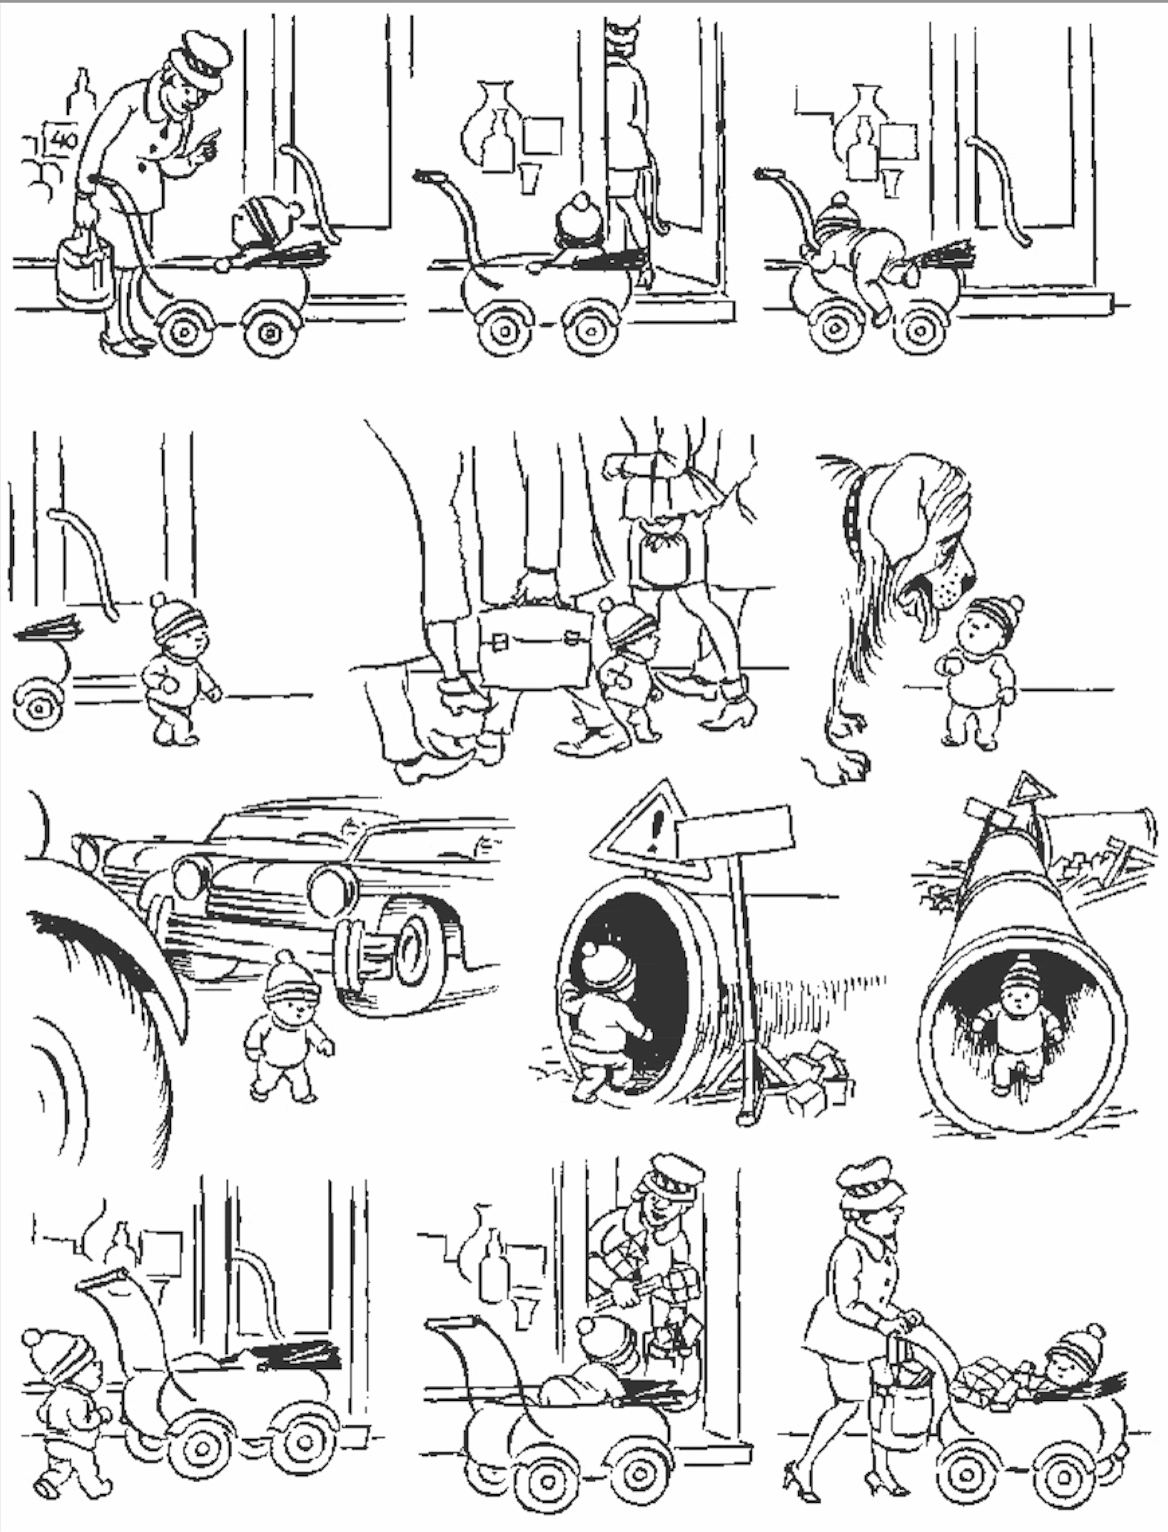
\includegraphics[width=\textwidth, center]{Figures/elicitation/adventure.png} 
\captionsetup{width=\textwidth}
\caption[Tasks: Adventure]{\label{fig:tasks:ad} The image used to elicit adventure task.}
\end{figure}

\begin{figure}[ht!]
    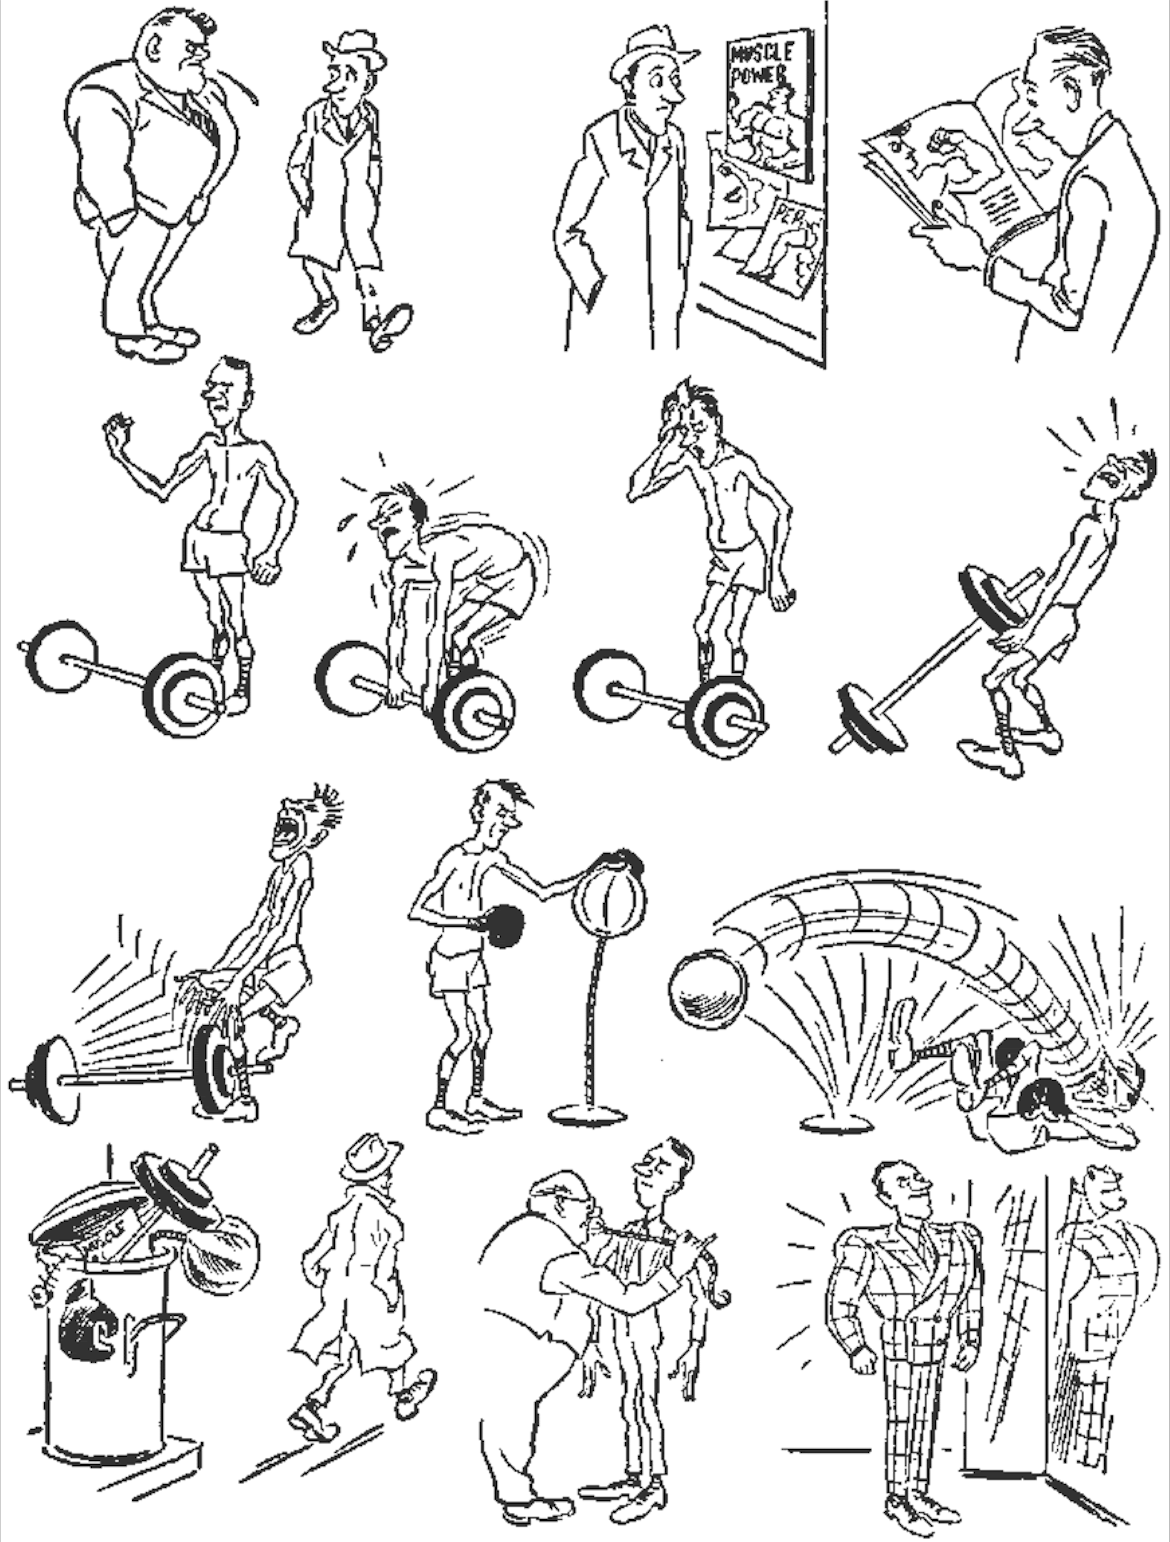
\includegraphics[width=\textwidth, center]{Figures/elicitation/sportsman.png} 
\captionsetup{width=\textwidth}
\caption[Tasks: Sportsman]{\label{fig:tasks:sp} The image used to elicit sportsman task.}
\end{figure}

\begin{figure}[ht!]
    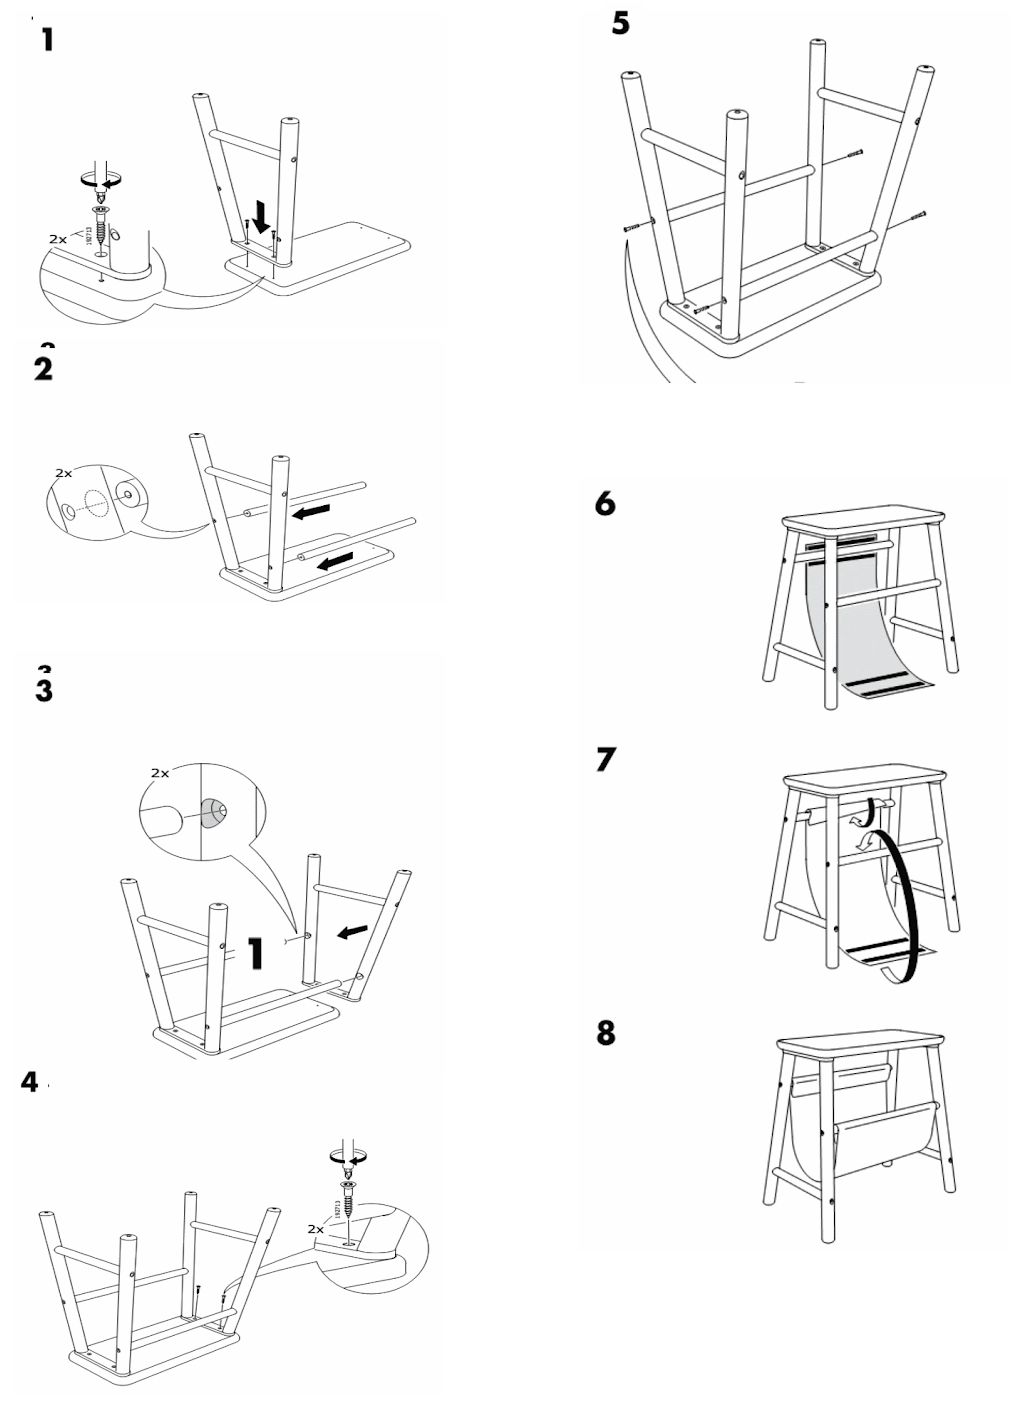
\includegraphics[width=\textwidth, center]{Figures/elicitation/chair.png} 
\captionsetup{width=\textwidth}
\caption[Tasks: Chair]{\label{fig:tasks:ch} The image used to elicit chair task.}
\end{figure}
%\include{Appendices/AppendixB}
%\include{Appendices/AppendixC}

%----------------------------------------------------------------------------------------
%	BIBLIOGRAPHY
%----------------------------------------------------------------------------------------

\printbibliography[heading=bibintoc]

%----------------------------------------------------------------------------------------

\end{document}  
